\documentclass[crop,tikz]{standalone}
\usepackage{graphicx}

% \usepackage{tikz}
\usetikzlibrary{3d,decorations.text,shapes.arrows,positioning,fit,backgrounds}
\usetikzlibrary{decorations.pathreplacing}
\usetikzlibrary{fadings}
\usetikzlibrary{arrows.meta} 
\usetikzlibrary{calc}

 % overleaf graphics path  
 \graphicspath{{CreateFigures/tikz/figures/}}
% \graphicspath{{/home/arefk/uio/MScThesis_AreKvanum2022_SeaIceML/CreateFigures/tikz/figures/}}
%-------------------- end preamble ----------------------

\begin{document}



\begin{tikzpicture}[x={(1,0)},y={(0,1)},z={({cos(60)},{sin(60)})},
  font=\sffamily\small, scale=.9]
  % \node [above] at (0,0) {a)};
  \node[inner sep=0pt] at (0,0) (sic) {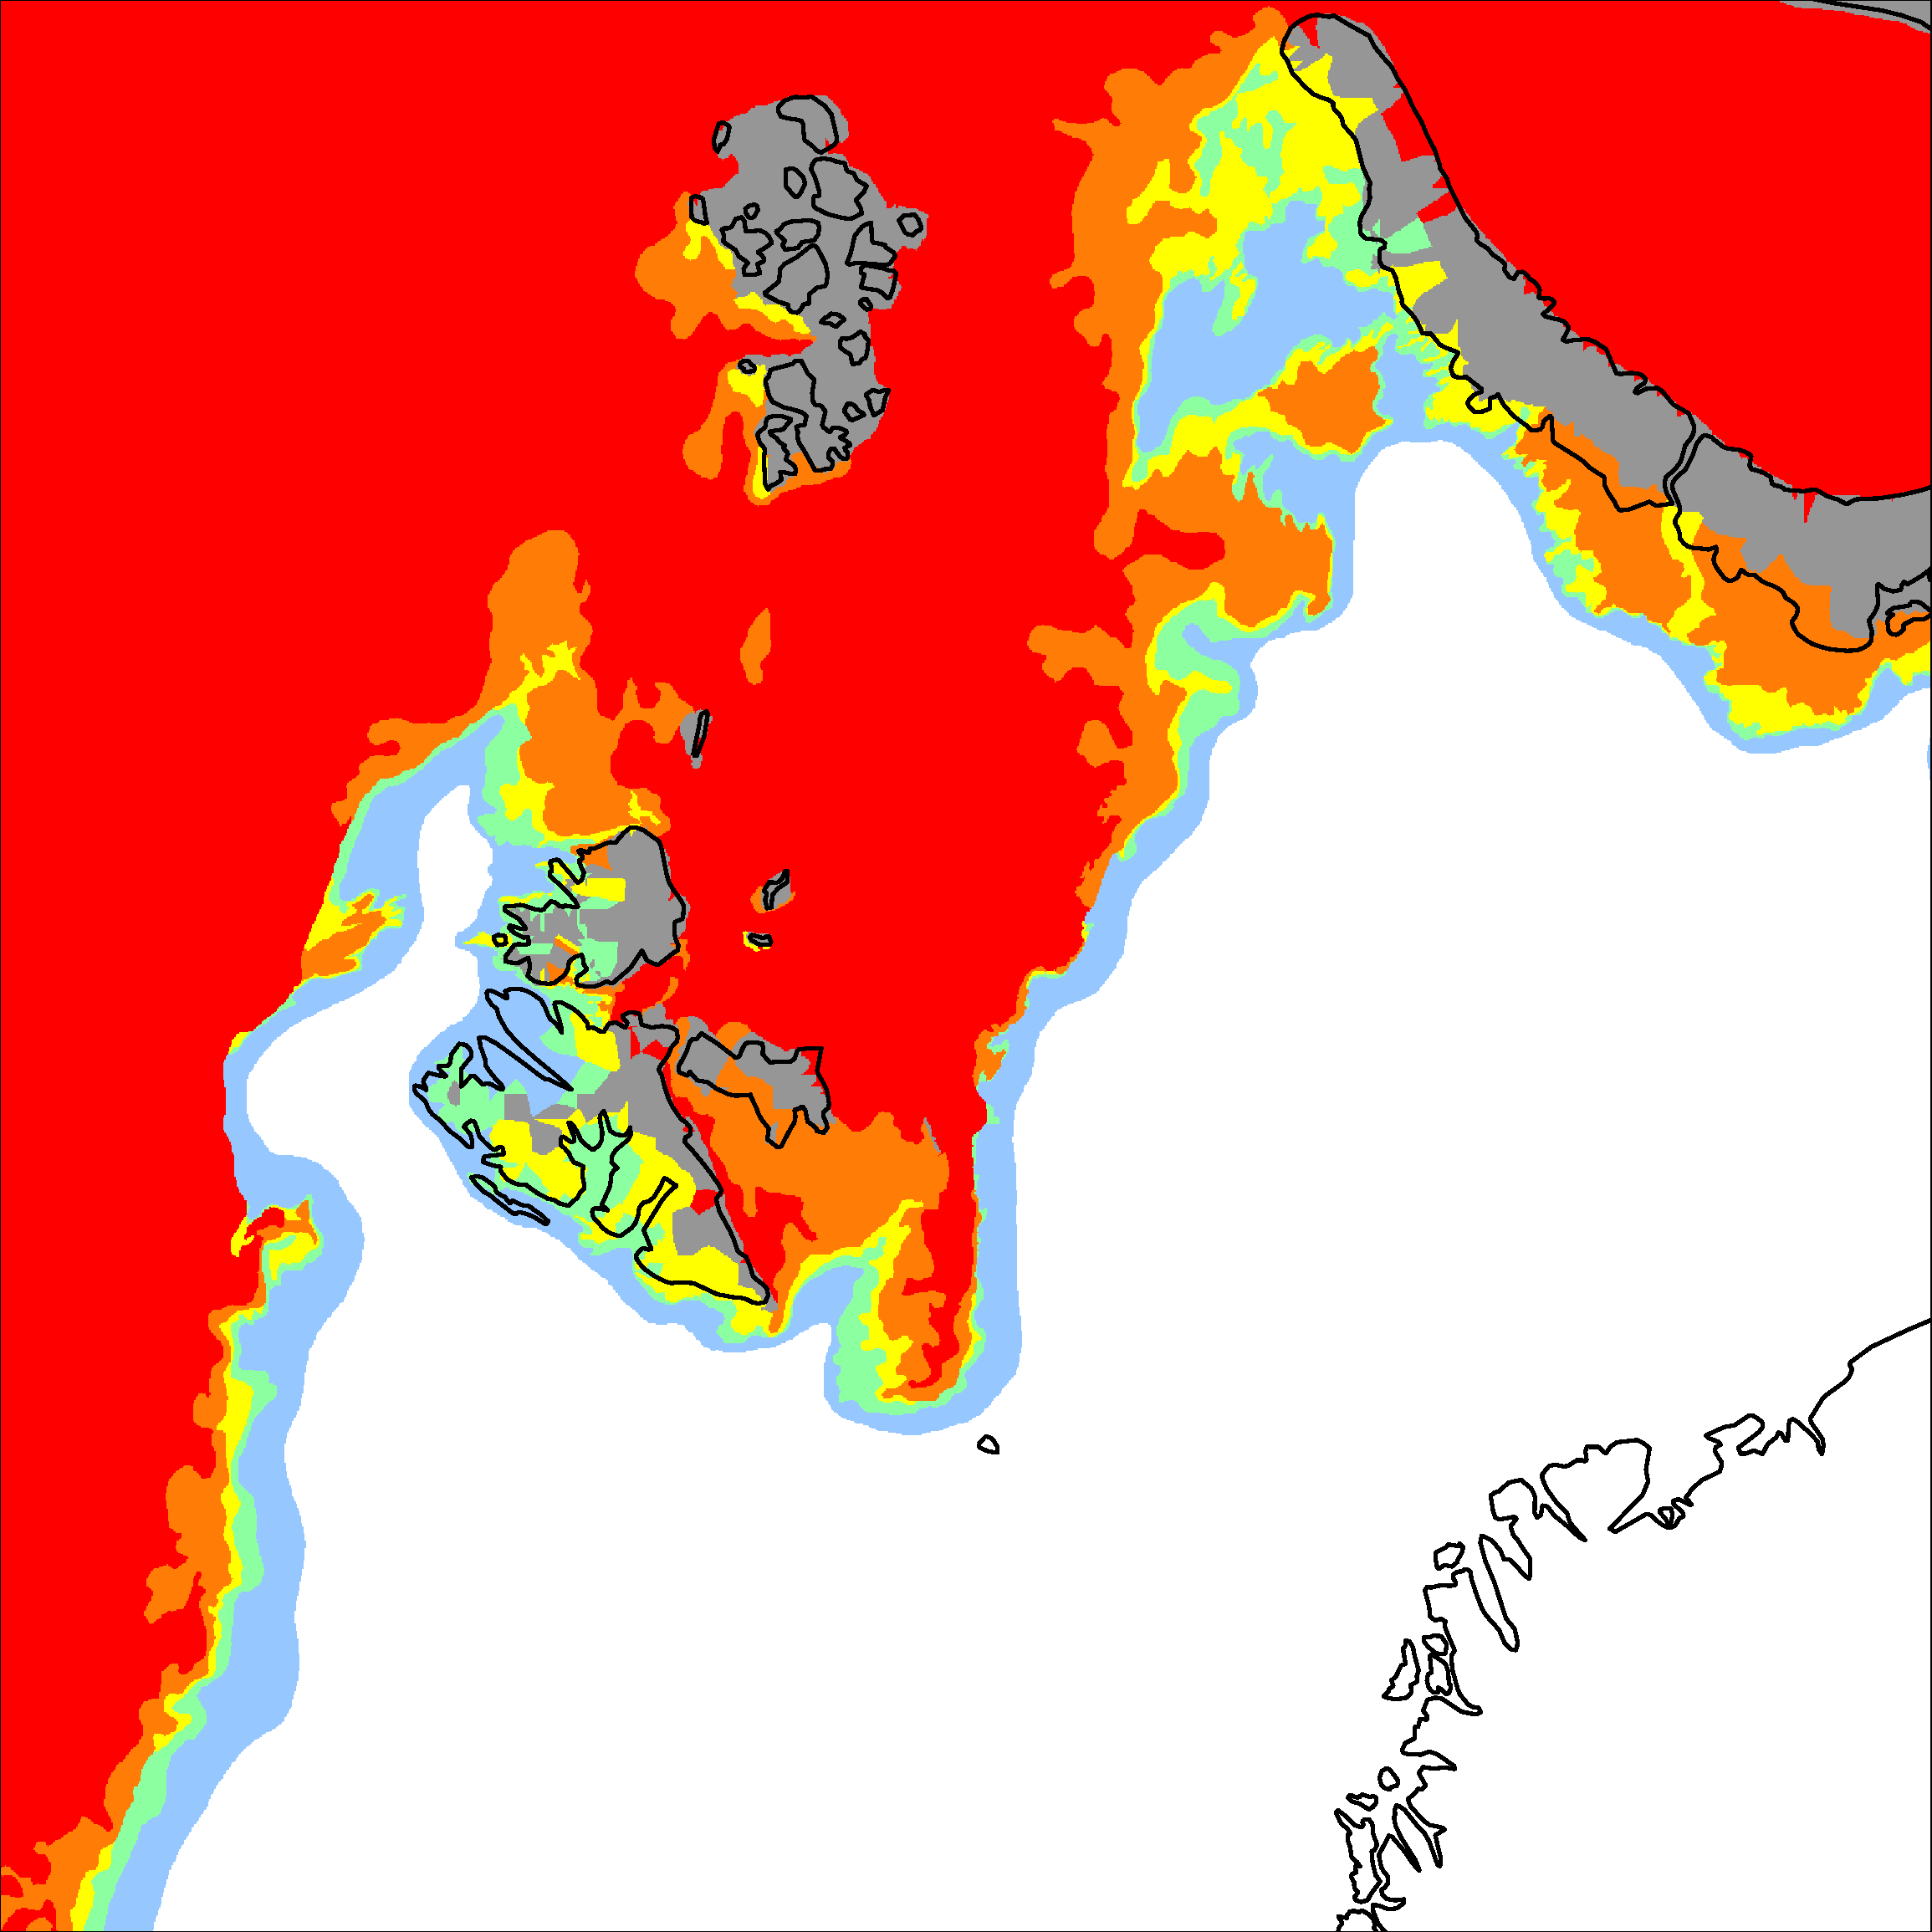
\includegraphics[width=.25\textwidth]{sic.pdf}};
  \node [above = 0.15cm of sic] (sic_name) {\large Recent Ice Chart};
  % \node [above] at (-6.5,.5) {b)};
  \node[right = 0.25cm of sic_name, align=center] (osi_name) {\large OSI-SAF SIC trend from \\ \large 5 previous days};
  \node (osi) at (sic -| osi_name) {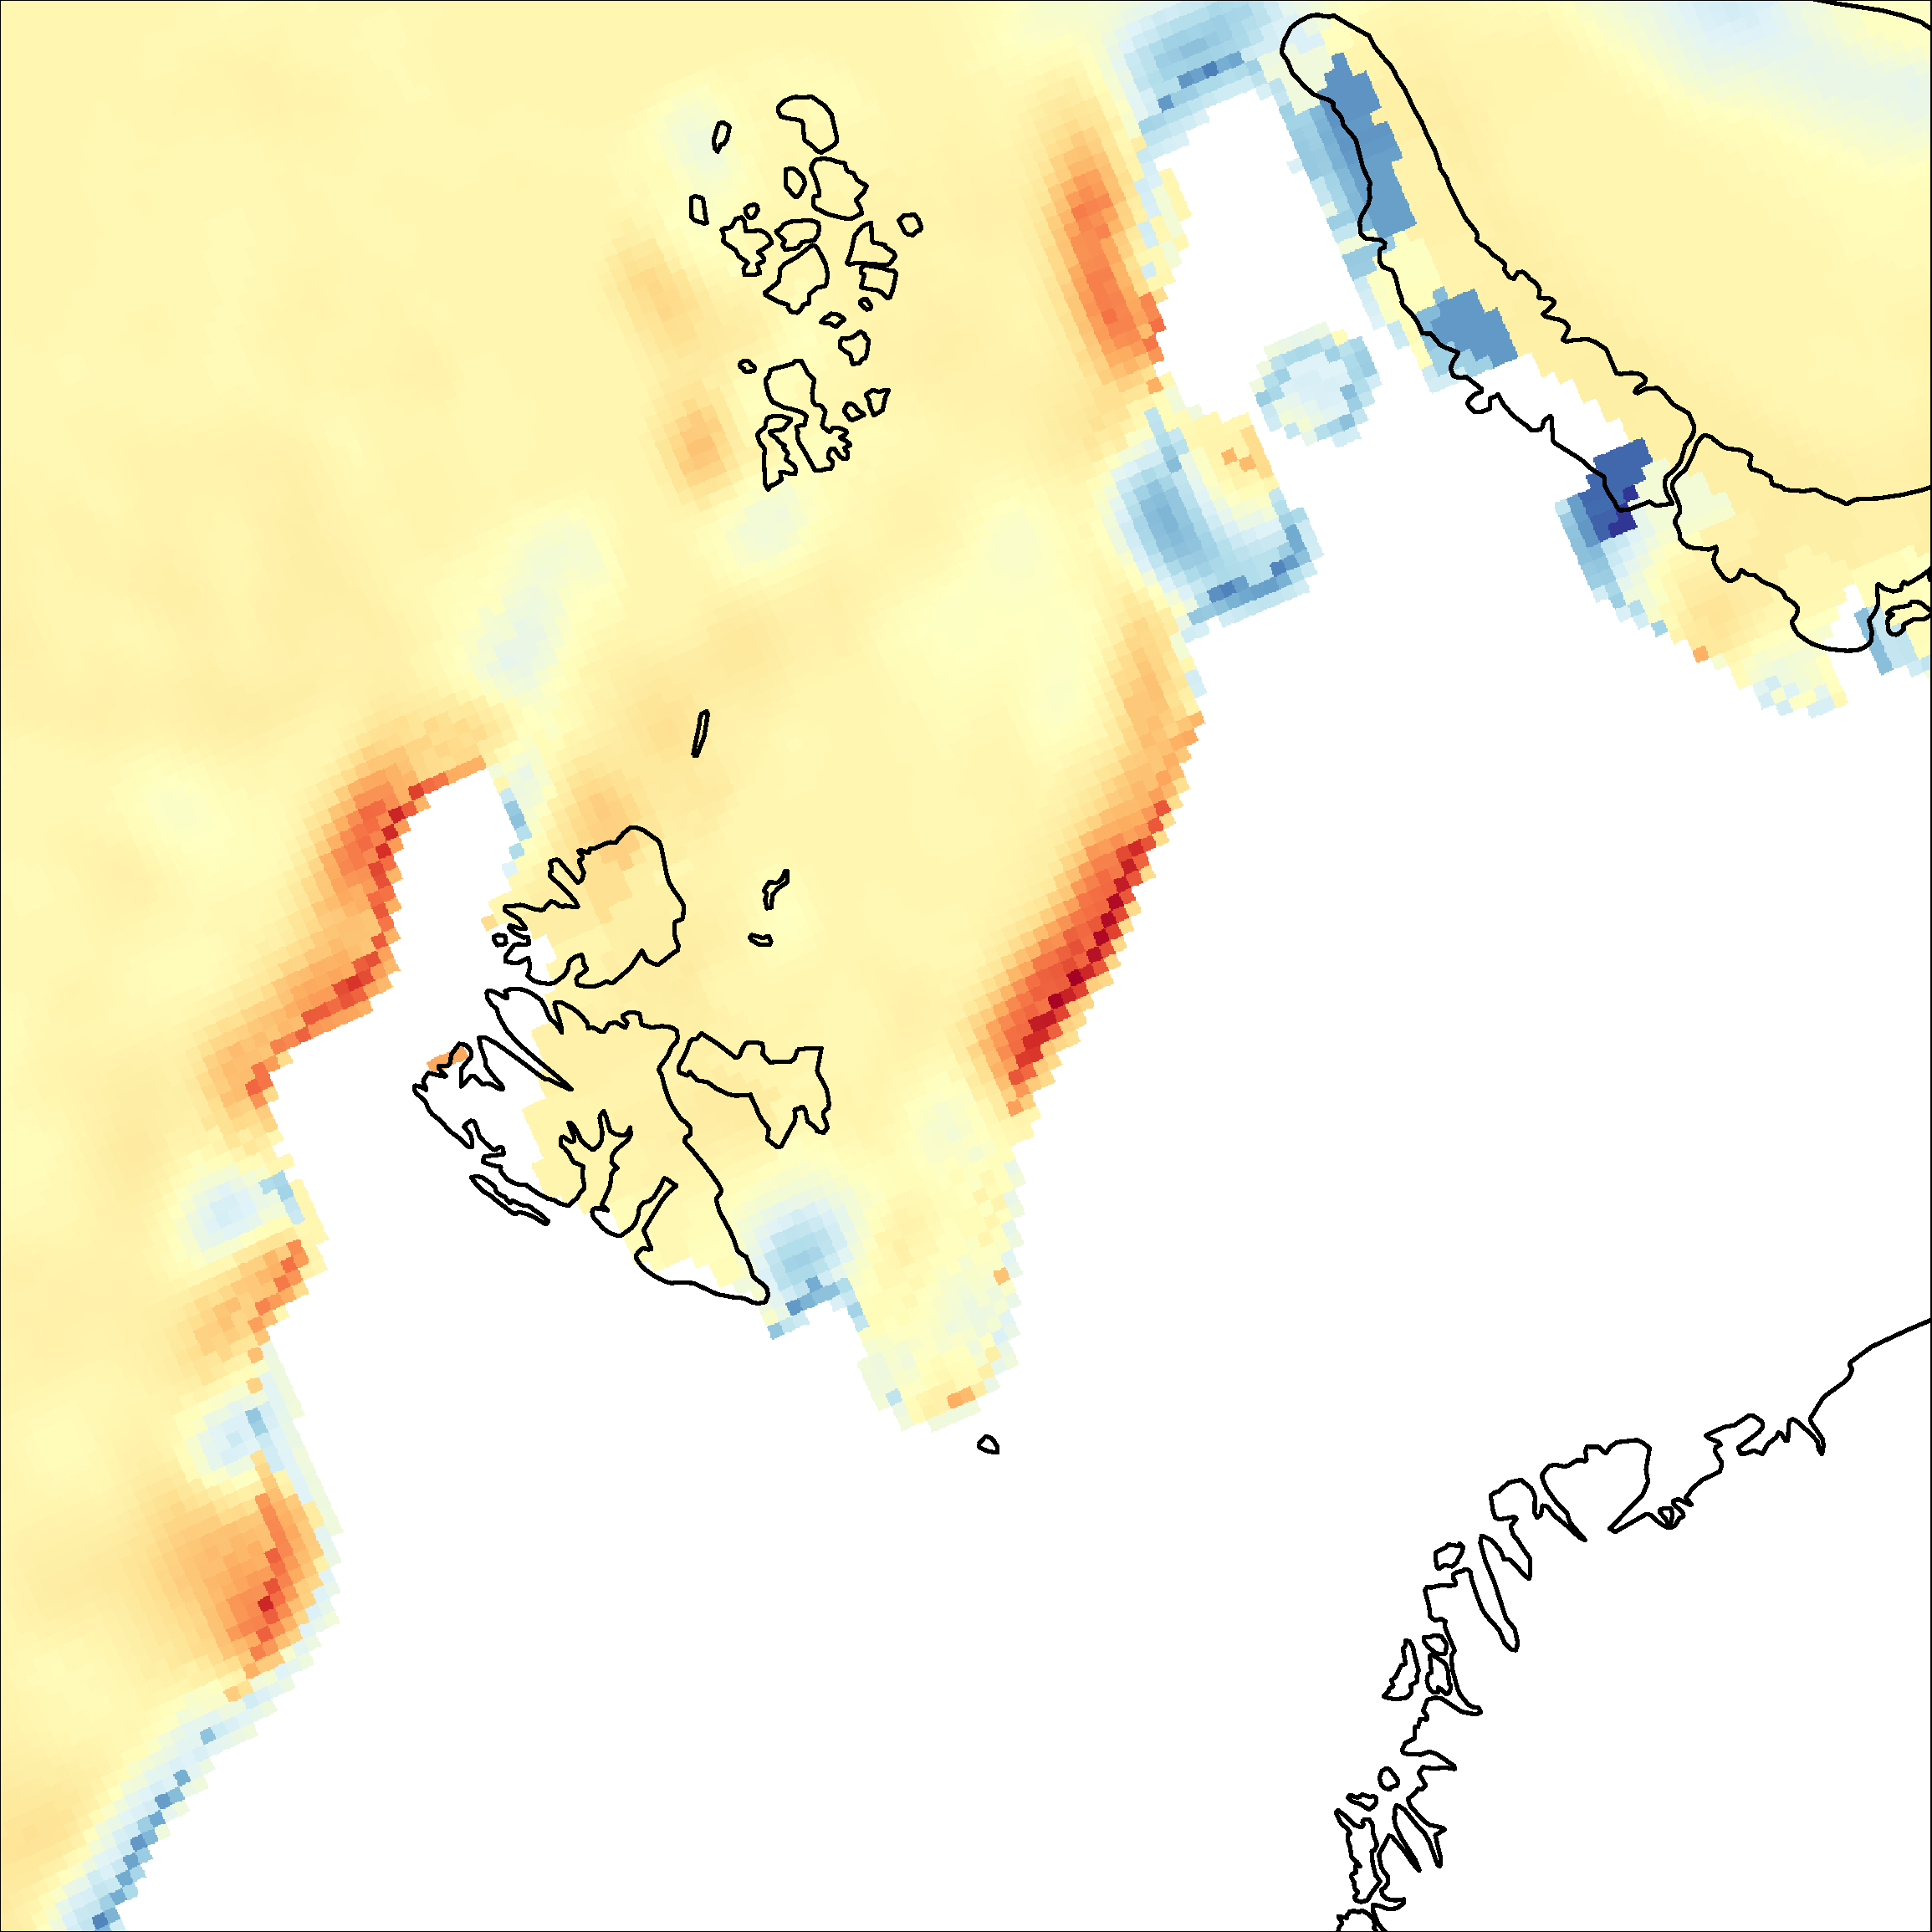
\includegraphics[width=.25\textwidth]{sic_trend.pdf}};
  % \node [above] at (-6.5,-1.4) {c)};
  \node[right = 0.25cm of osi_name, align = center] (arome_name) {\large AROME Arctic \\ \large t2m and wind forecasts};
  
  \node (aa_forecasts) at (sic -| arome_name) {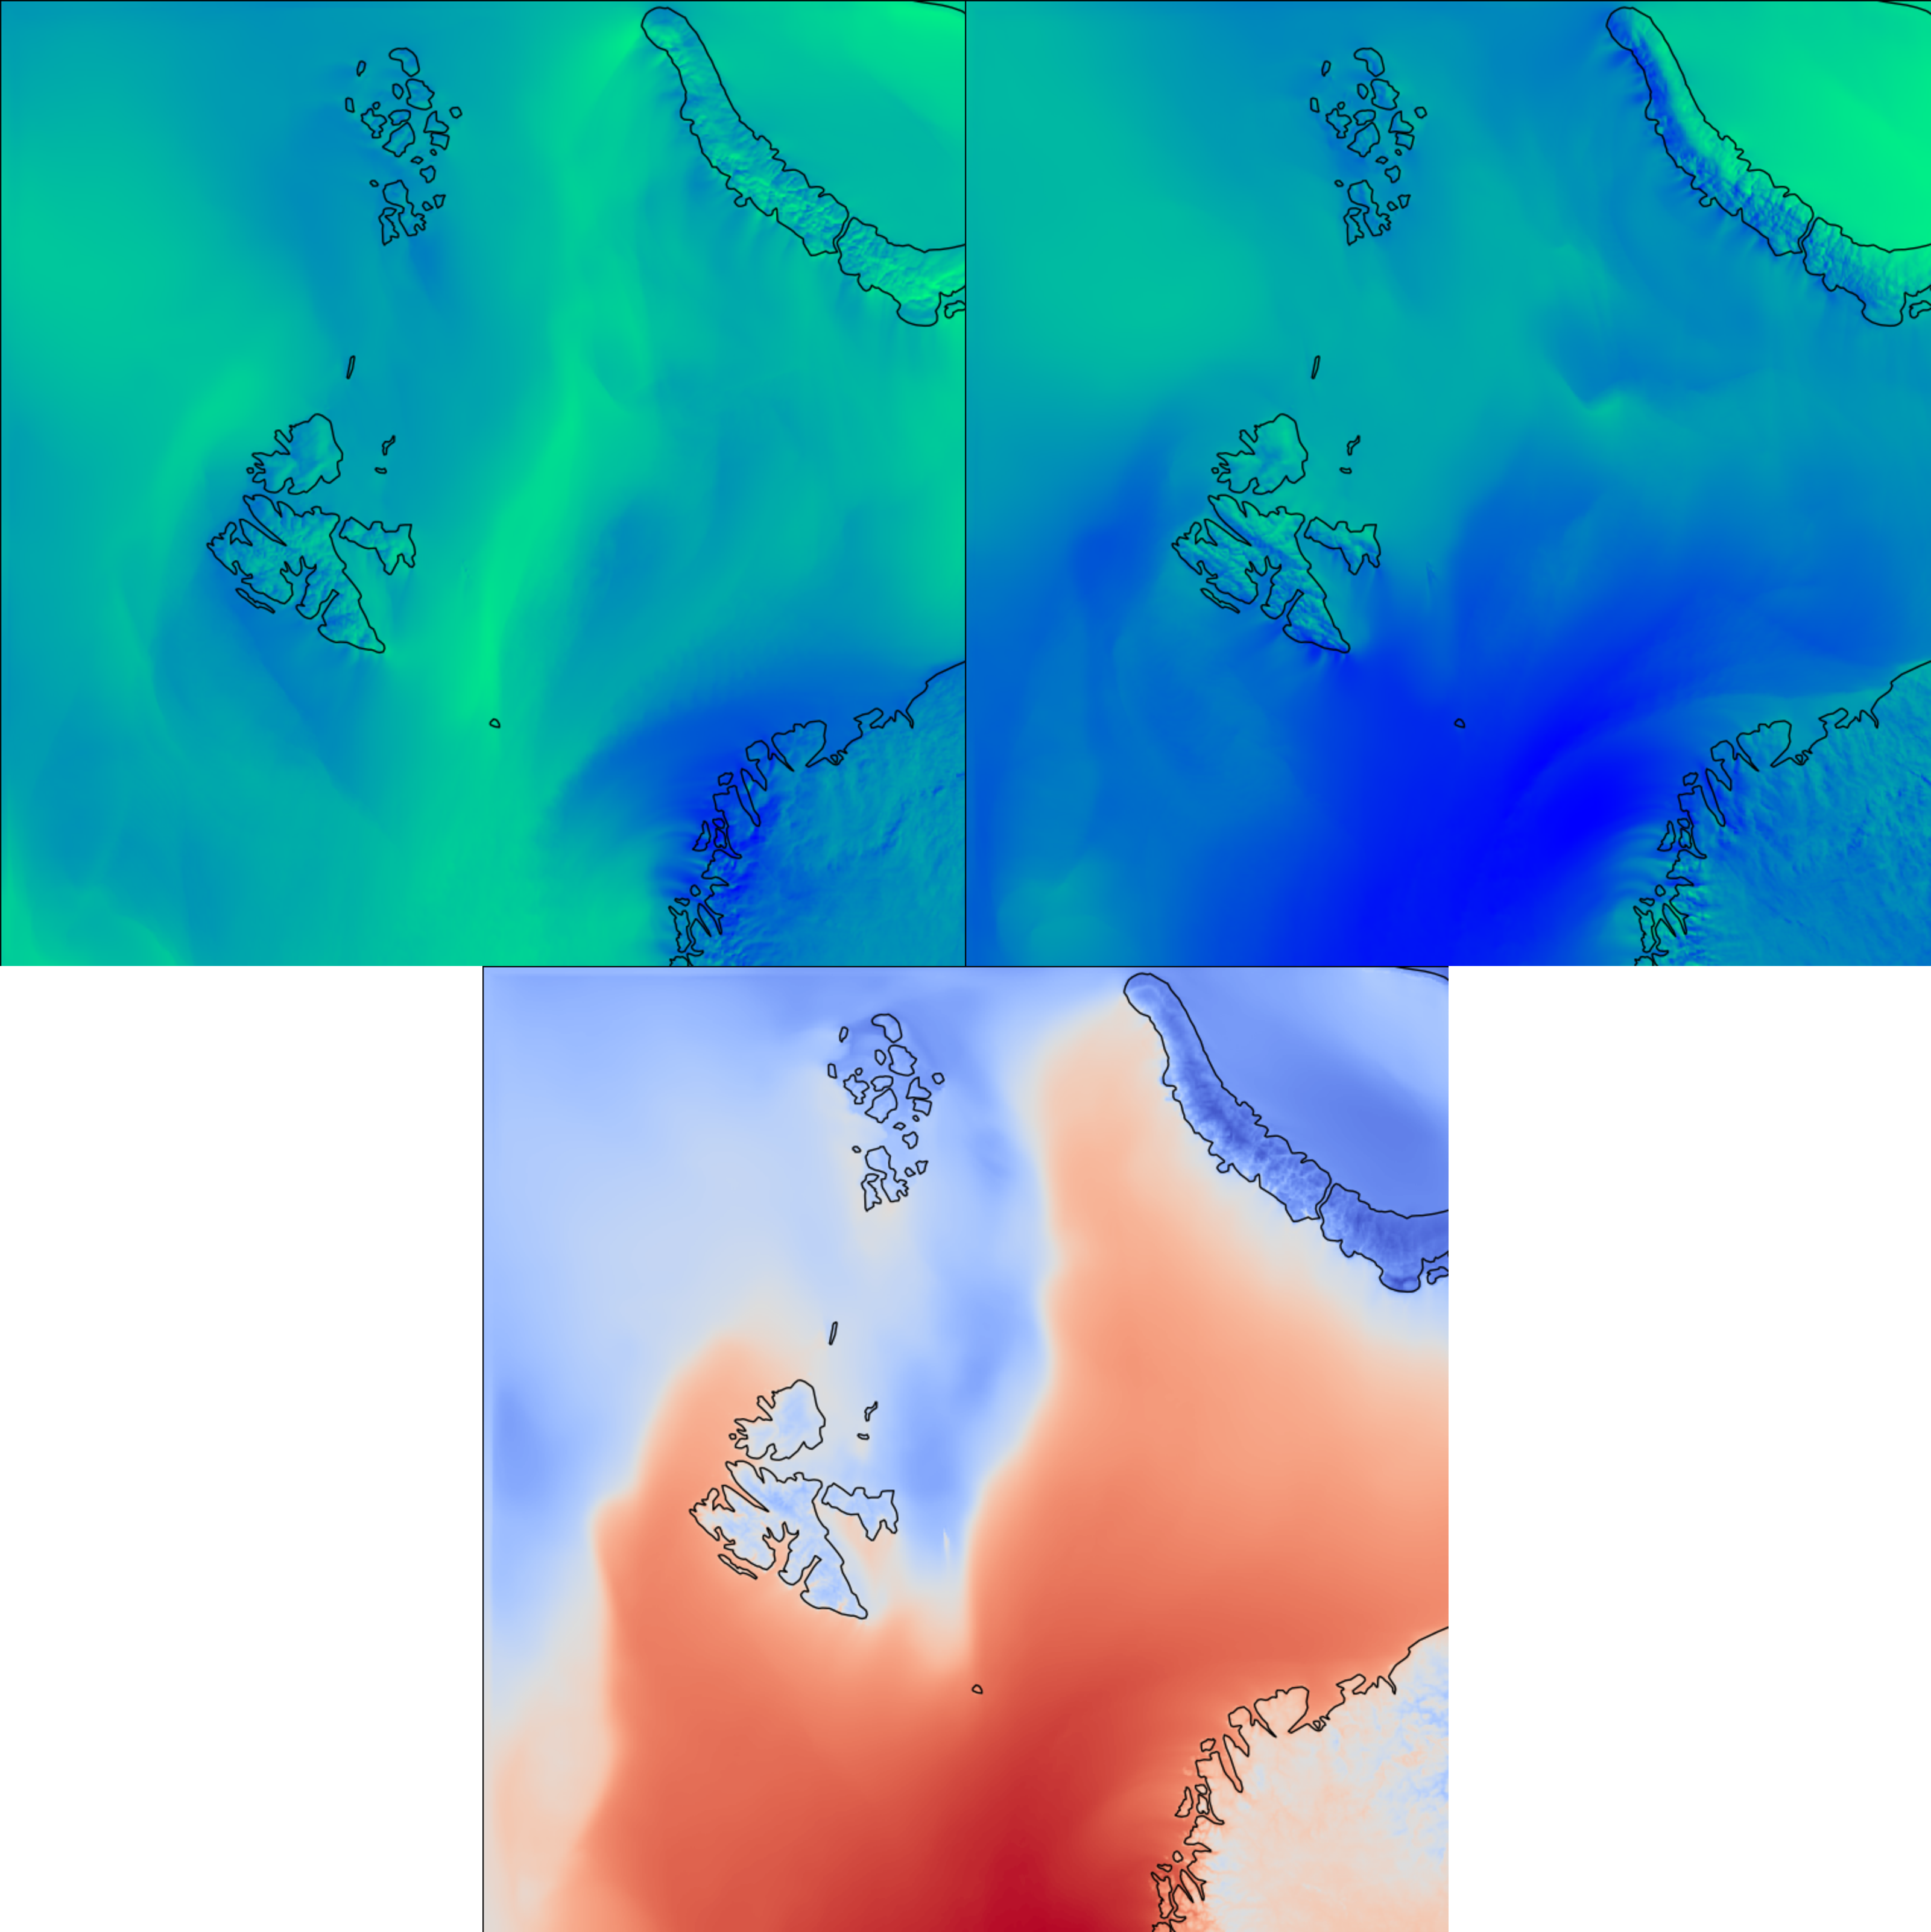
\includegraphics[width=.25\textwidth]{gimp_arome_stack.pdf}};

  \node[right = 0.25cm of arome_name, align = center] (mask_name) {\large Land-Sea Mask};
  \node (aa_mask) at (sic -| mask_name) {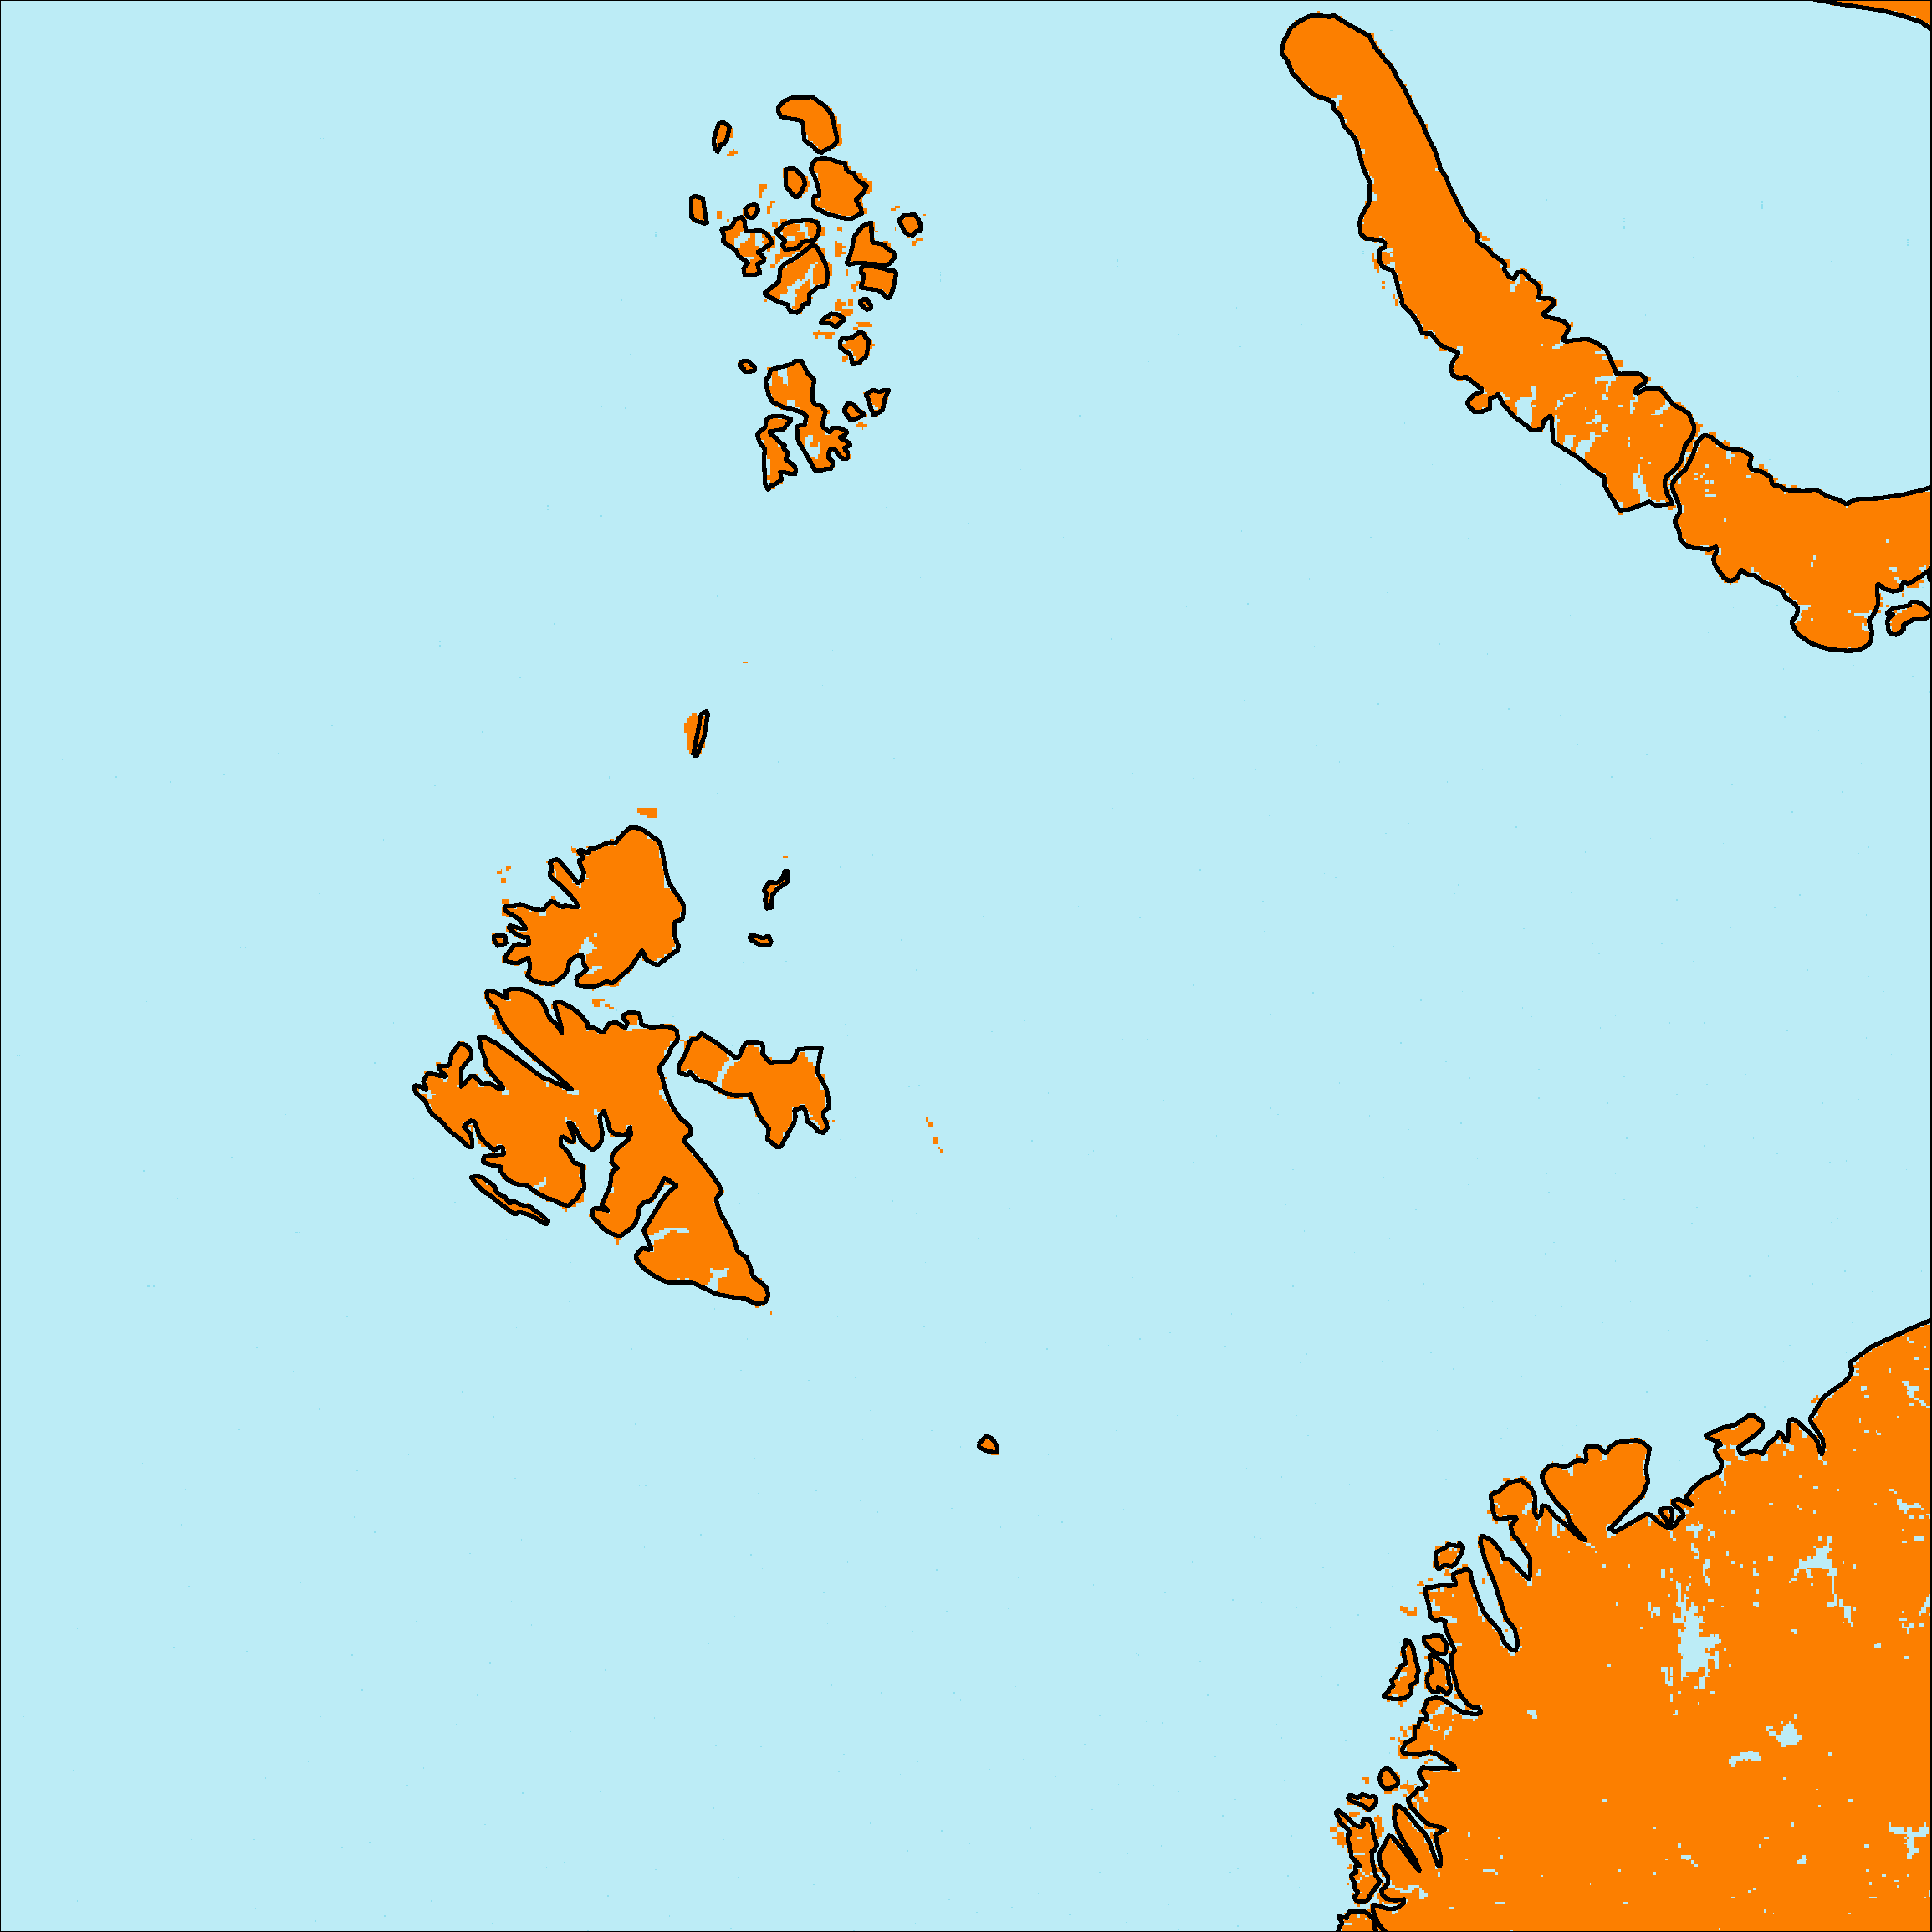
\includegraphics[width=.25\textwidth]{lsmask.pdf}};
  % \node[draw,single arrow, black,fill=black!30] at (-1.25,0.5,0) {INPUT};
  
  \coordinate[yshift=-5cm] (sample_stack) at ($(osi)!0.5!(aa_forecasts)$);
  \draw [line width=0.8mm, -{Stealth[length=8mm, round]}, shorten >=1.75cm, shorten <=0.2cm]
          (sic.south) -- (sample_stack);

  \draw [line width=0.8mm, -{Stealth[length=8mm, round]}, shorten >=1.4cm, shorten <= 0.1cm]
          (osi.south) -- (sample_stack);

  \draw [line width=0.8mm, -{Stealth[length=8mm, round]}, shorten >=1.4cm, shorten <= 0.1cm]
          (aa_forecasts.south) -- (sample_stack);
  
  \draw [line width=0.8mm, -{Stealth[length=8mm, round]}, shorten >=1.75cm, shorten <=0.2cm]
          (aa_mask.south) -- (sample_stack);

  \node at (sample_stack) (stack1) {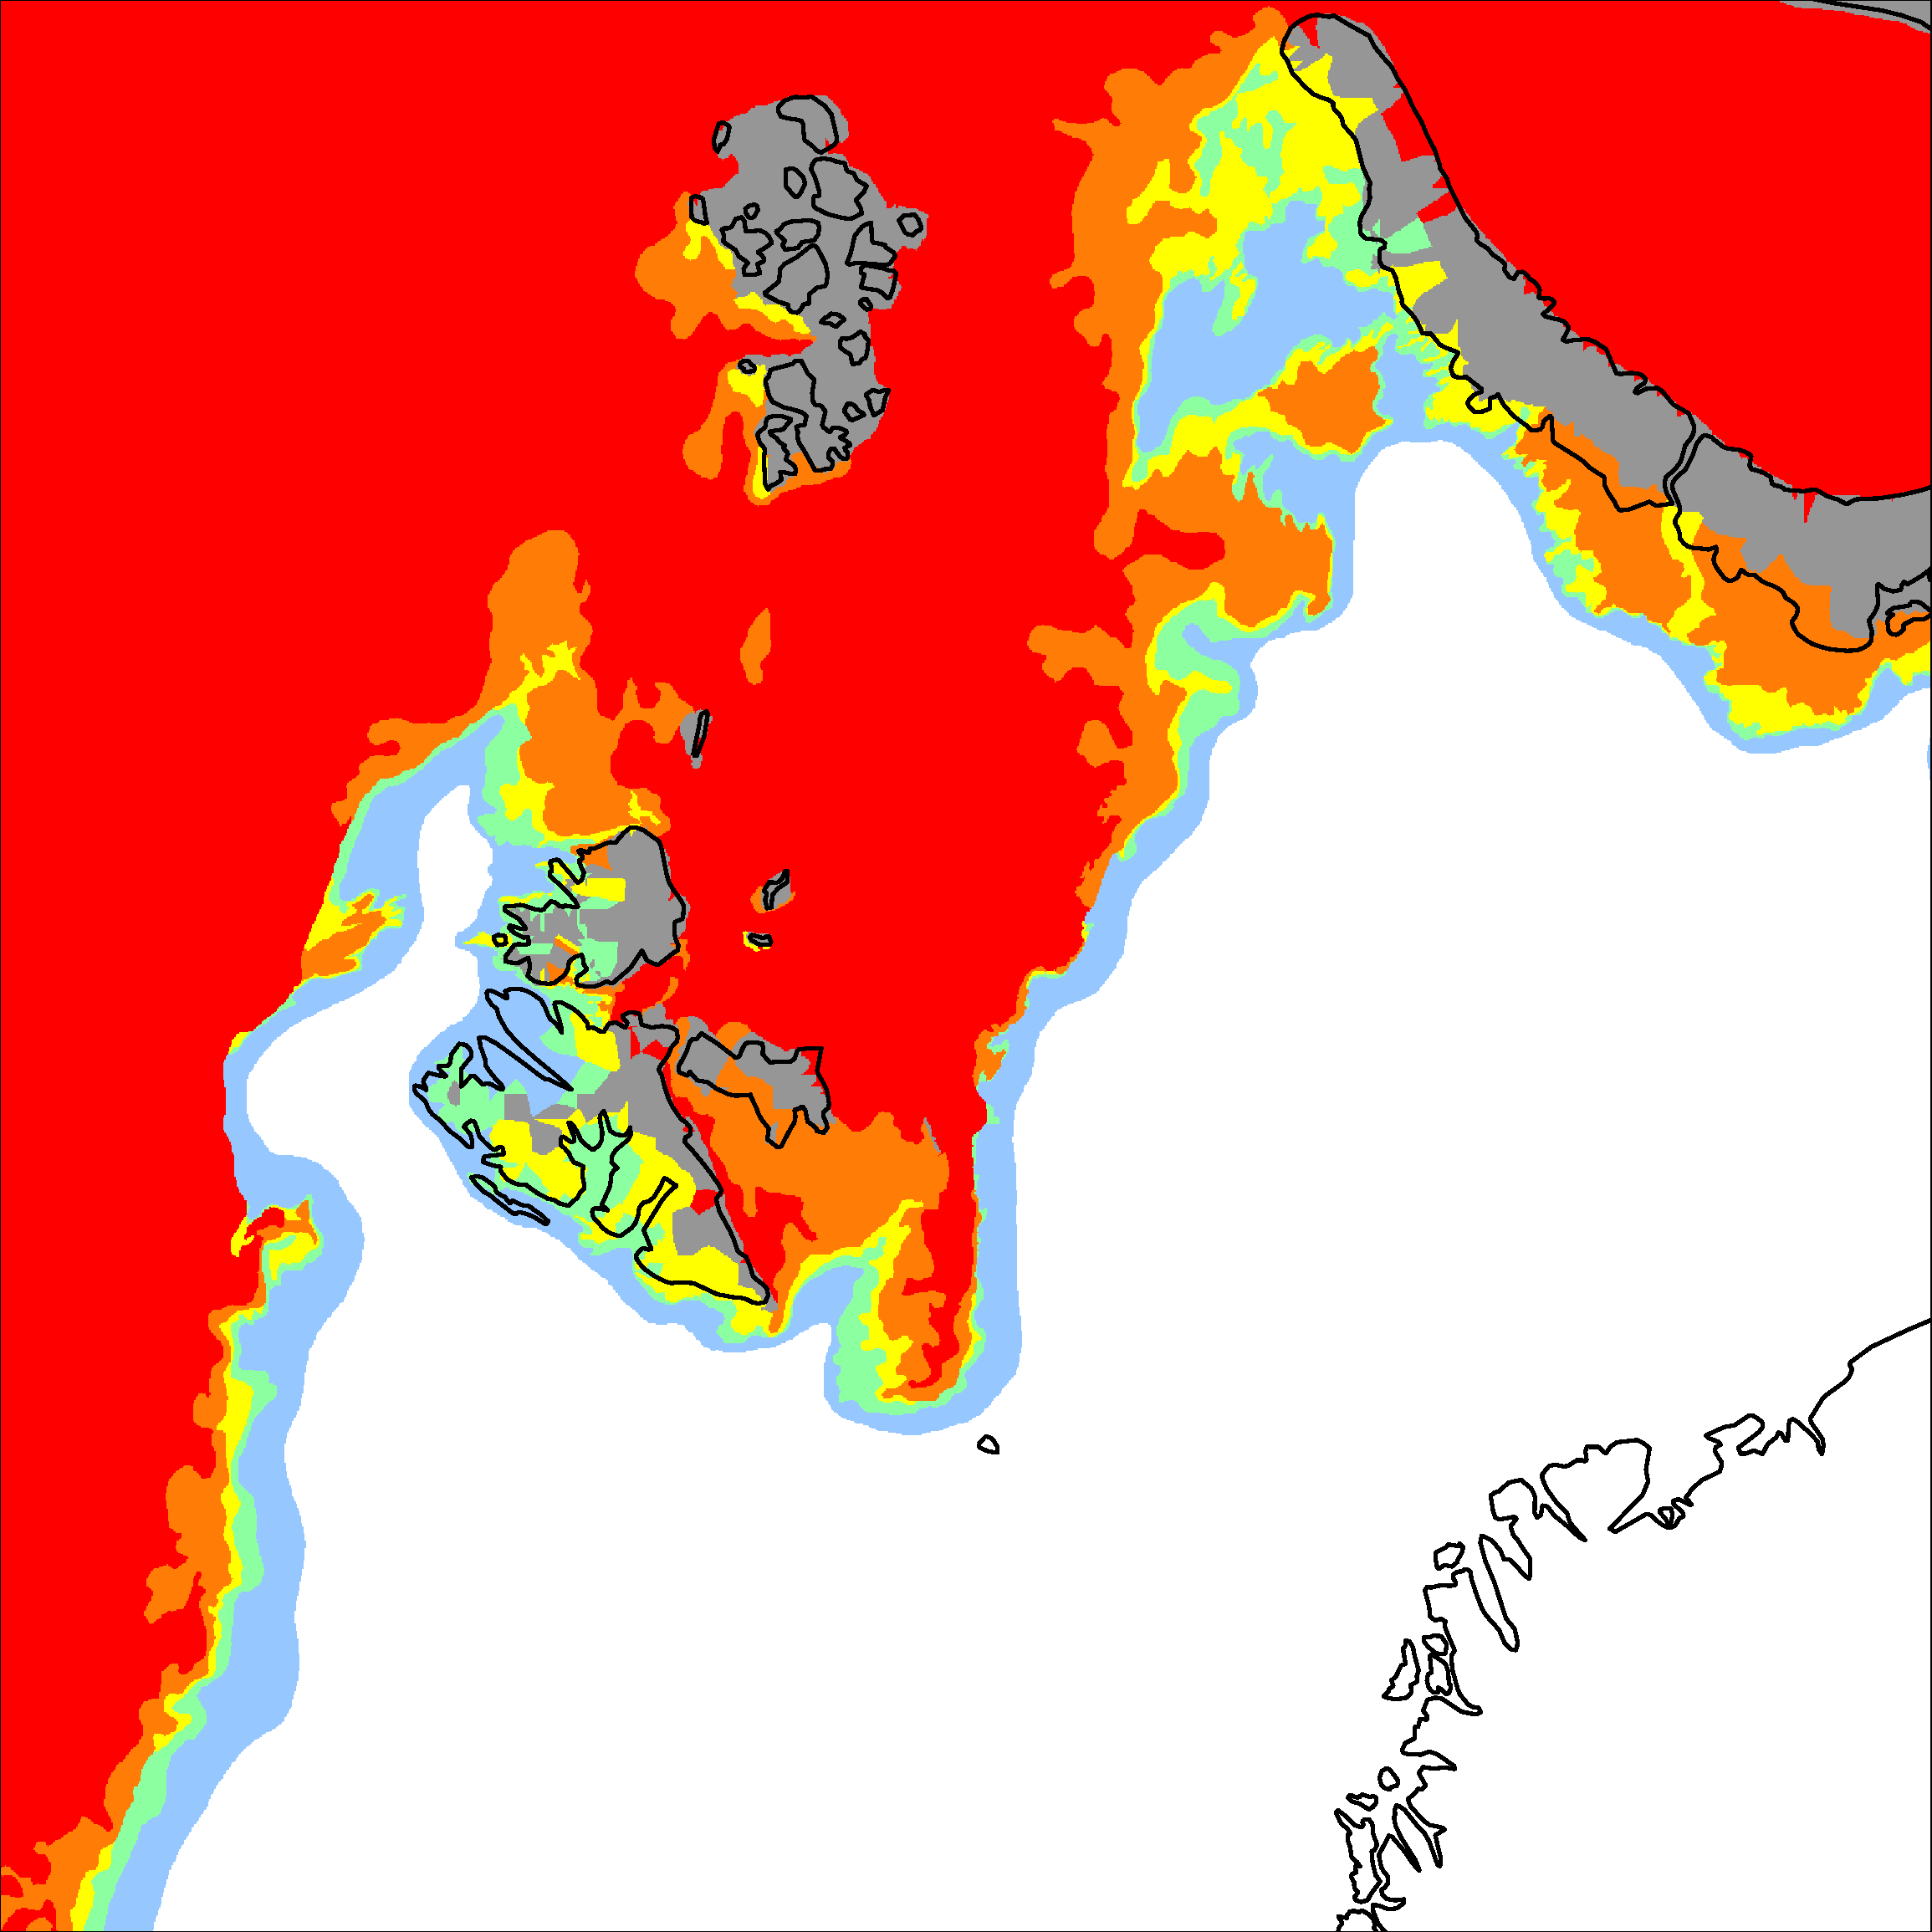
\includegraphics[width=.15\textwidth]{sic.pdf}};
  \node[yshift = -0.1cm, xshift = 0.1cm] at (sample_stack) (stack2) {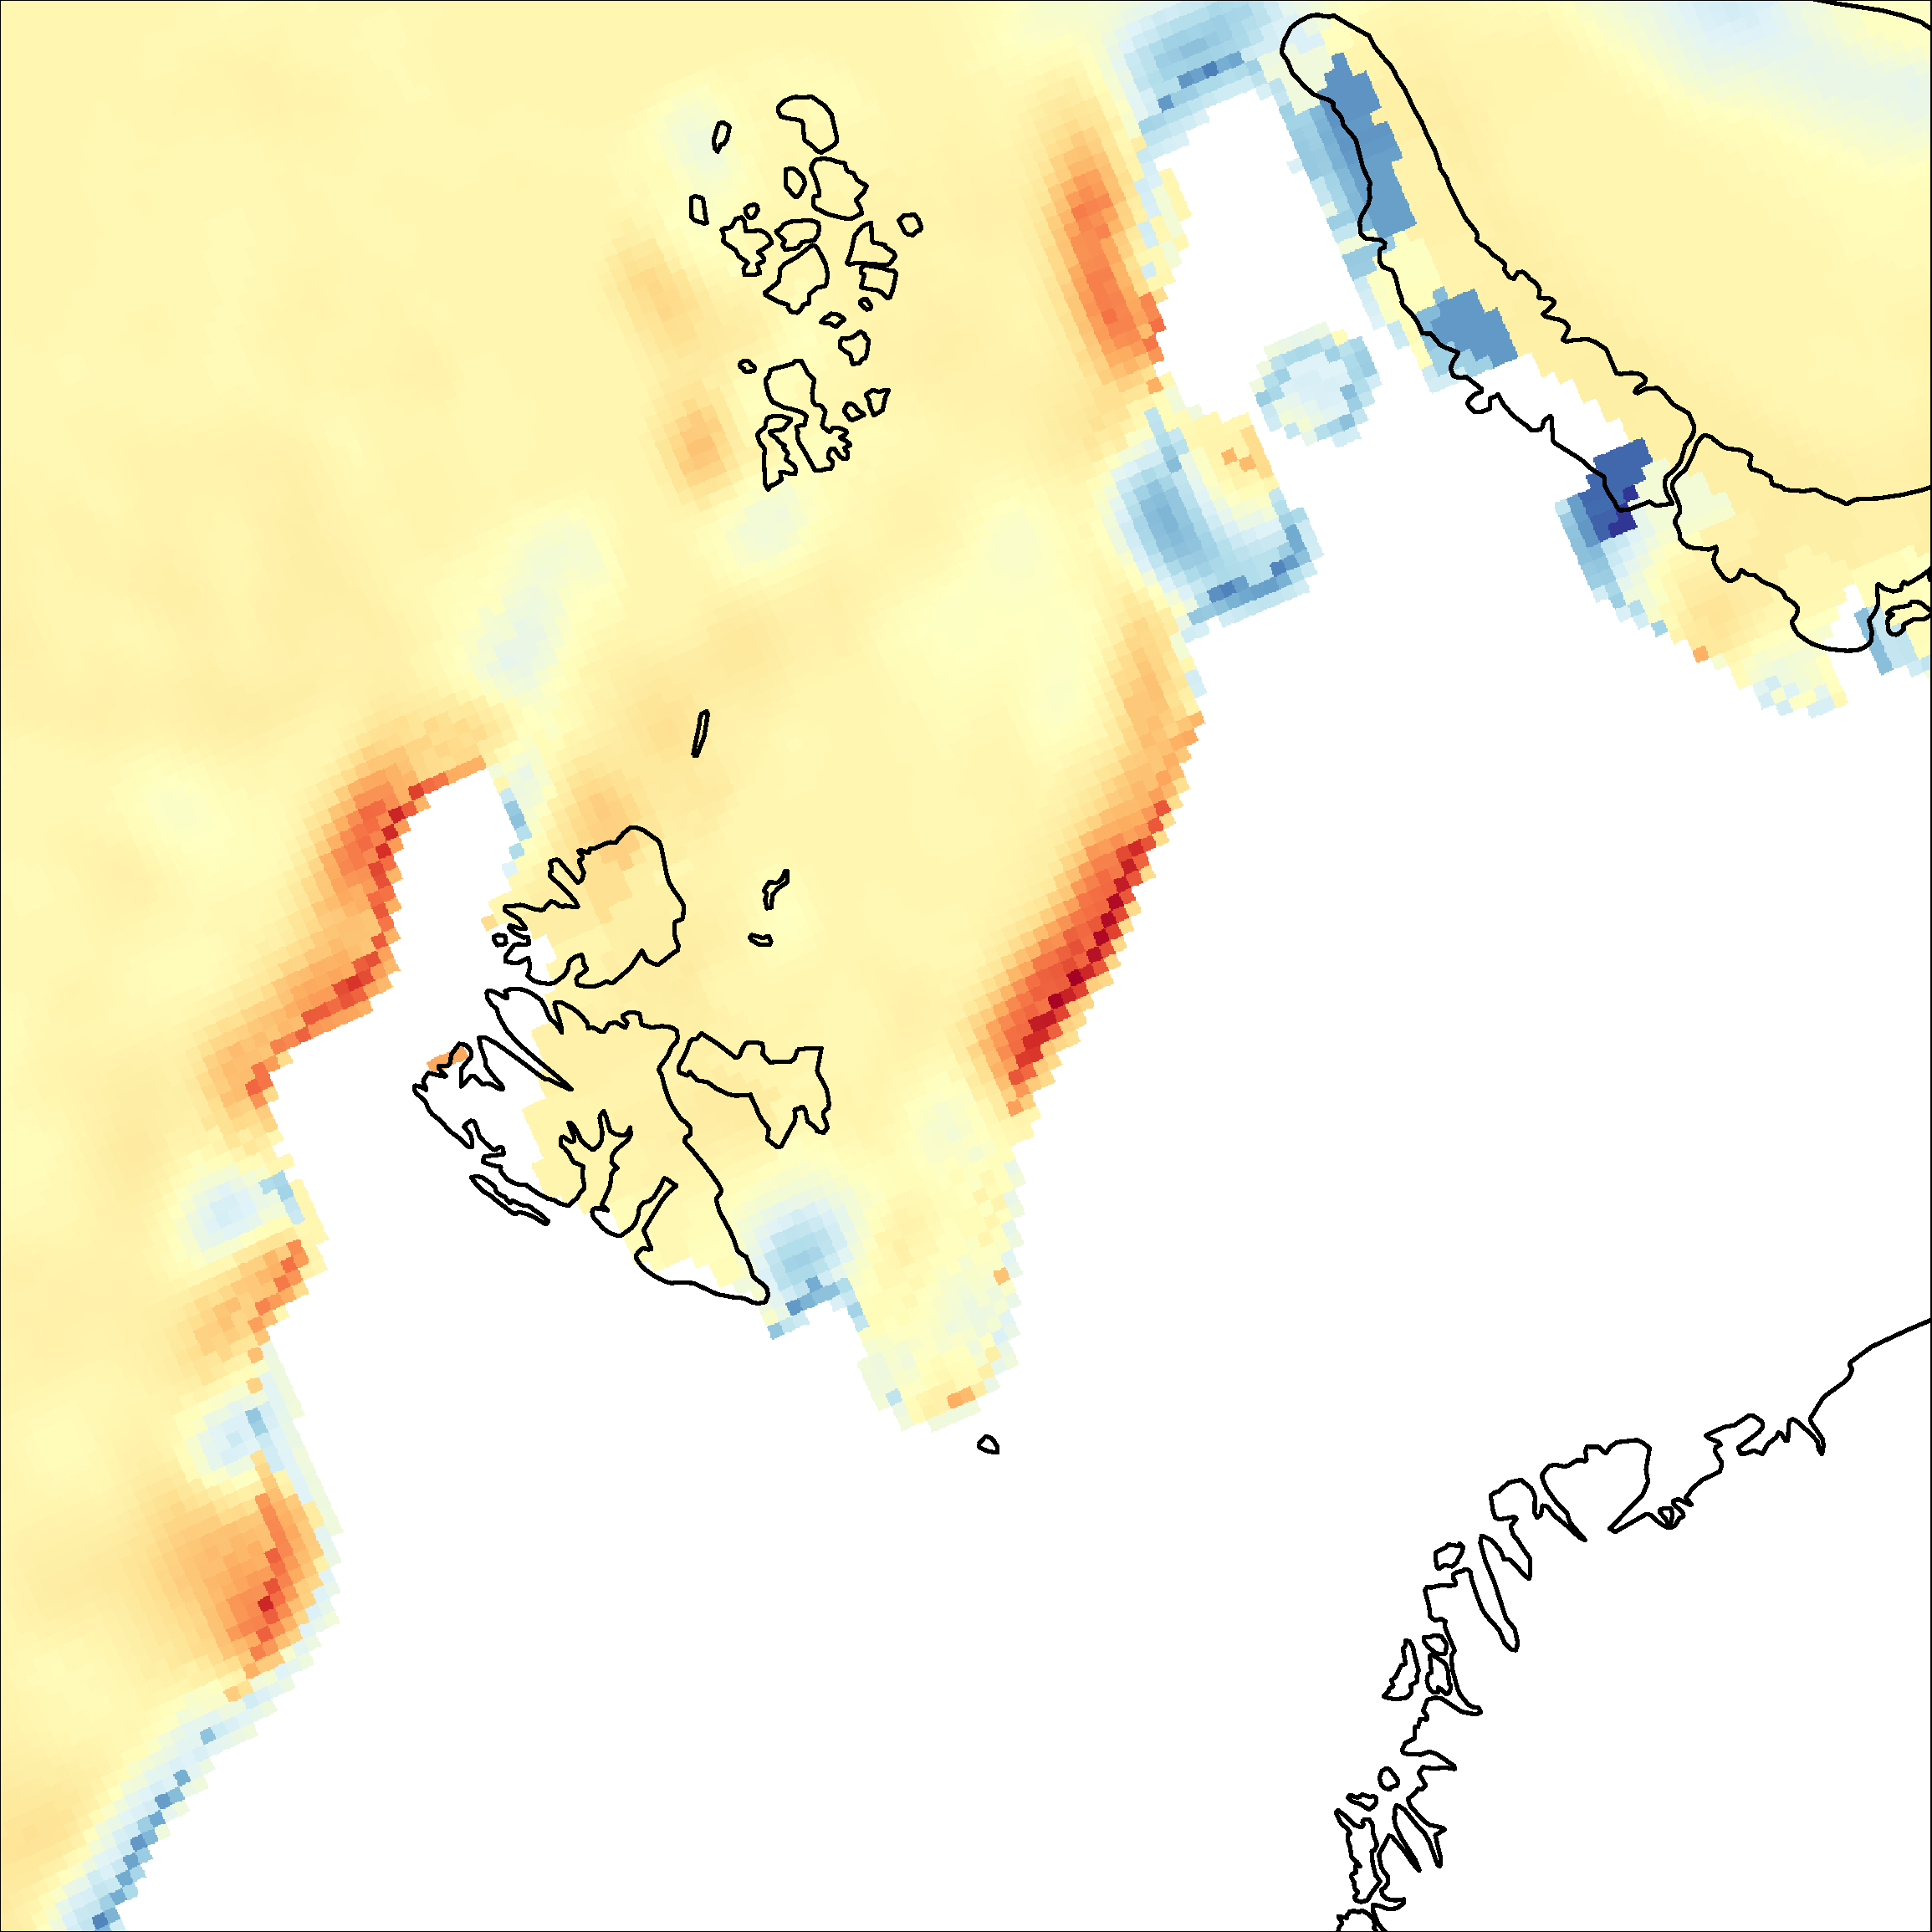
\includegraphics[width=.15\textwidth]{sic_trend.pdf}};
  \node[yshift = -0.2cm, xshift = 0.2cm] at (sample_stack) (stack3) {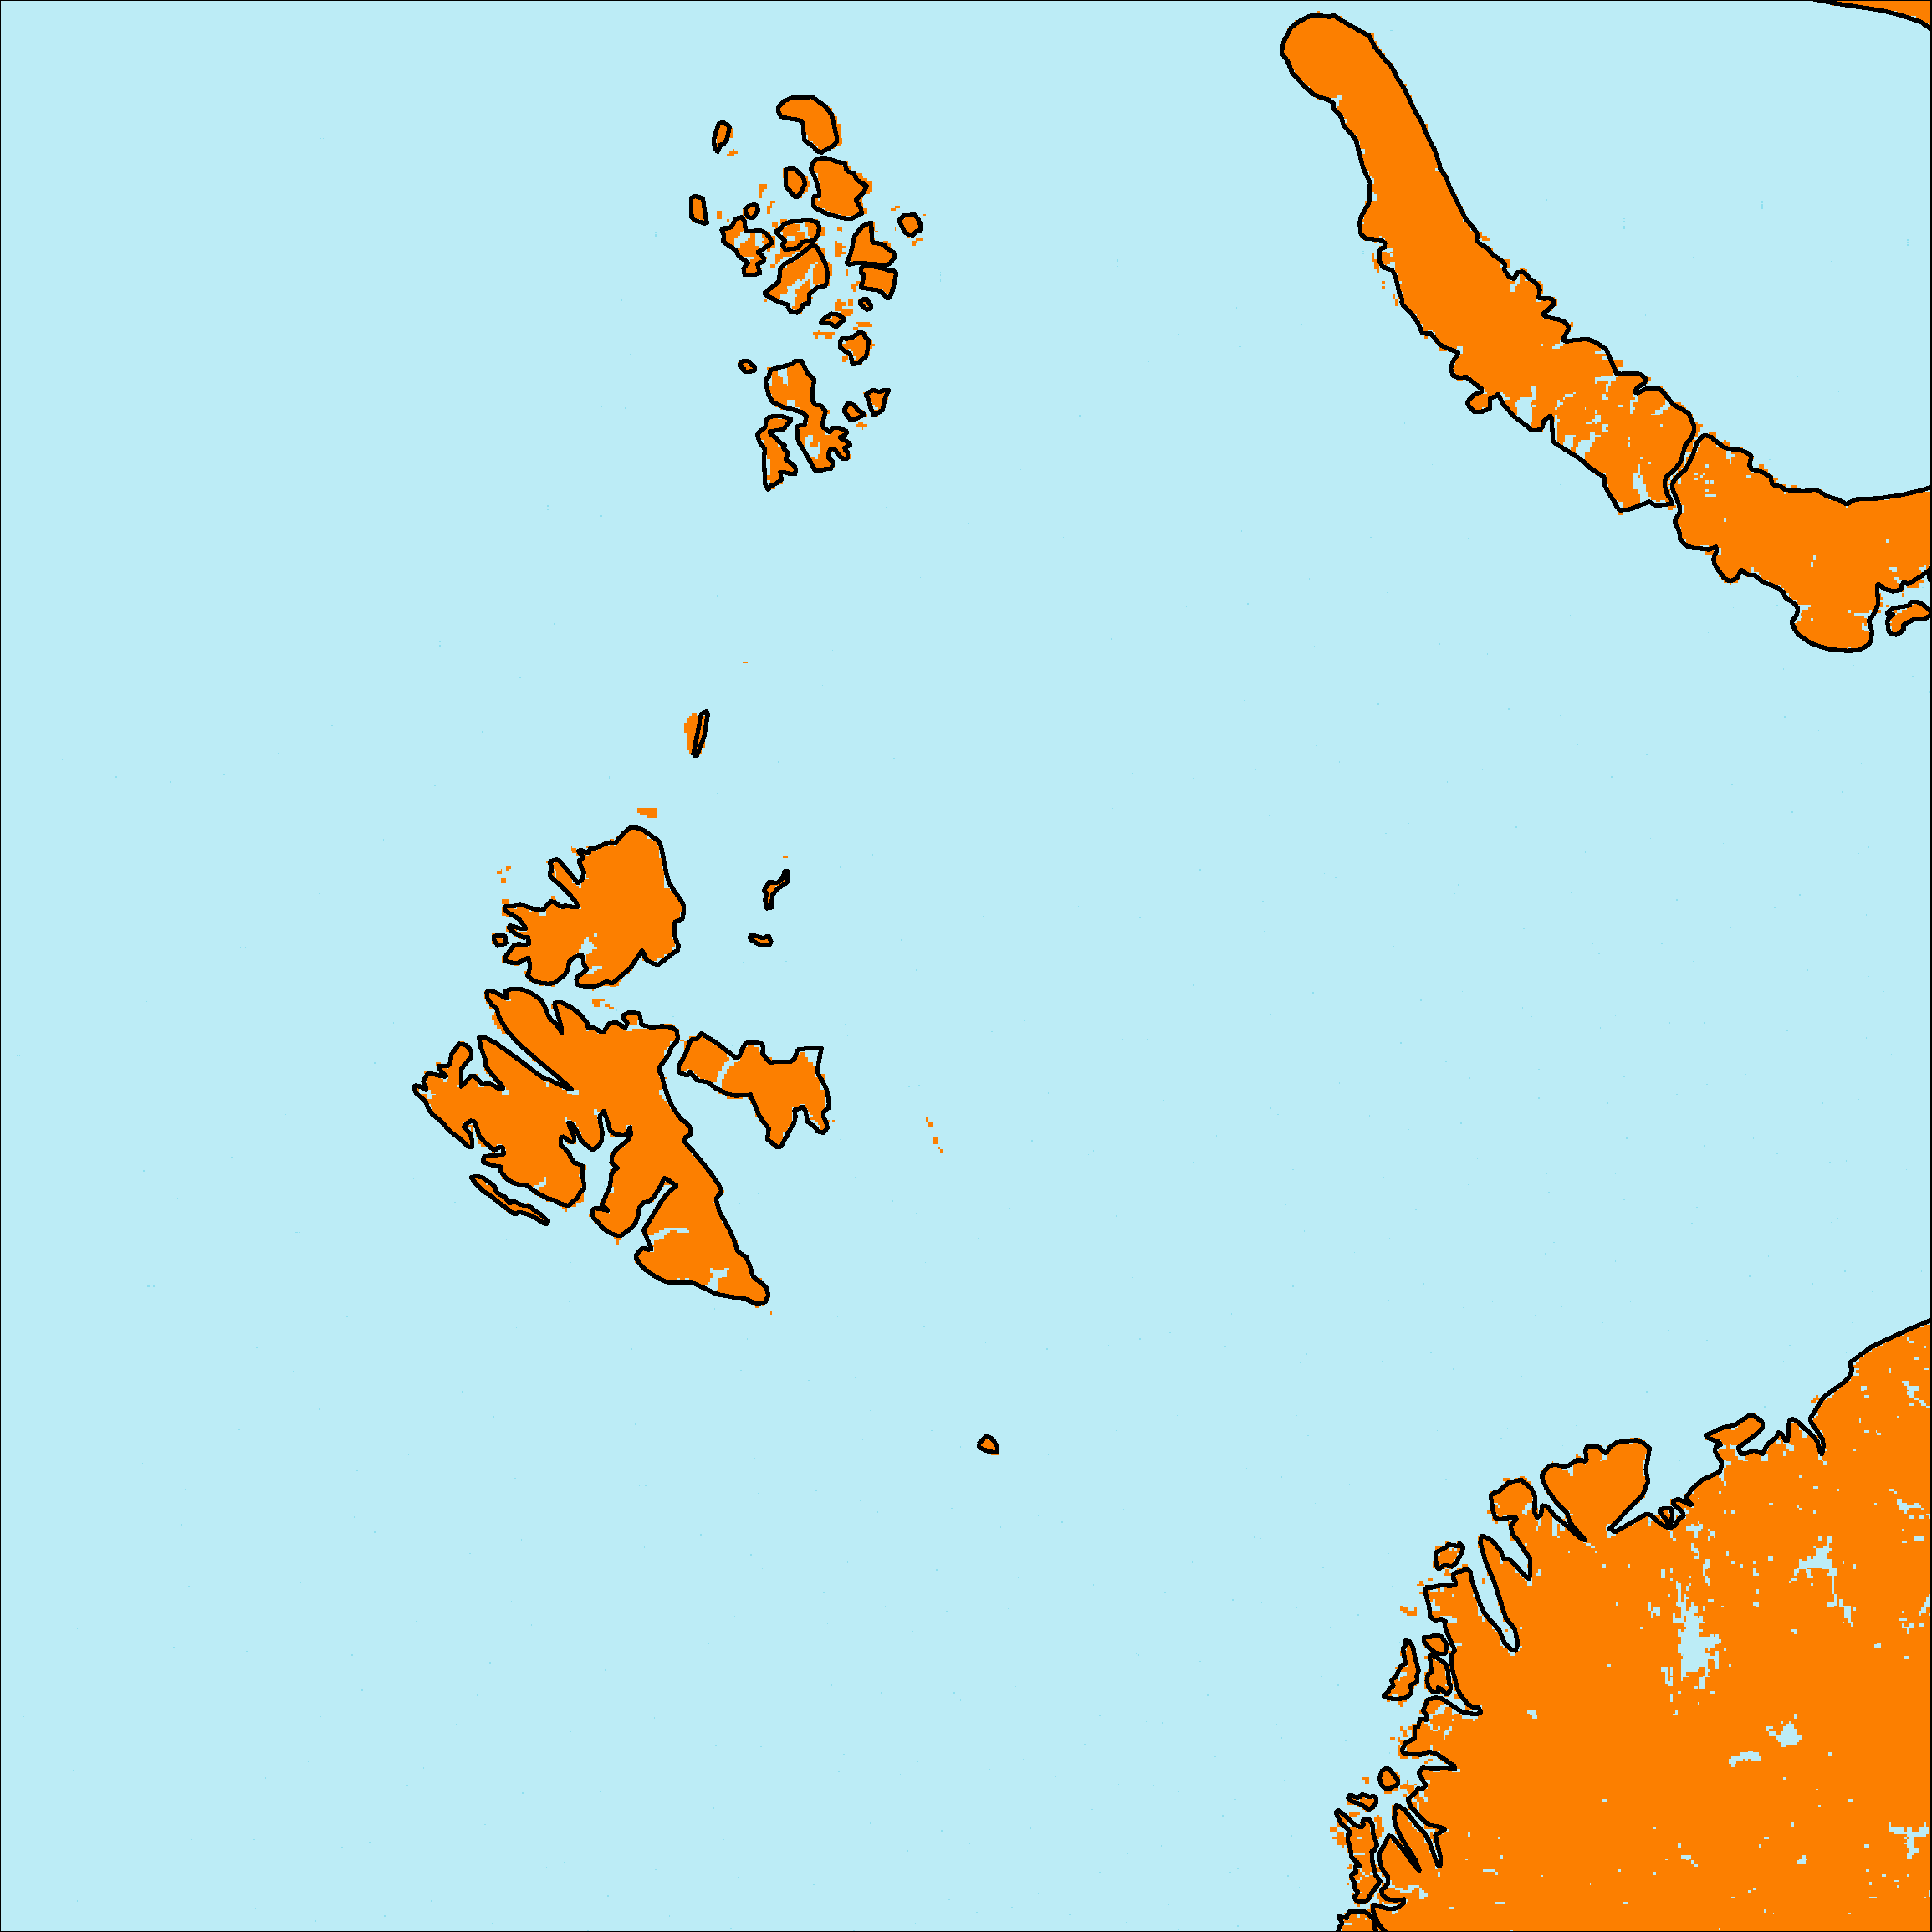
\includegraphics[width=.15\textwidth]{lsmask.pdf}};
  \node[yshift = -0.3cm, xshift = 0.3cm] at (sample_stack) (stack4) {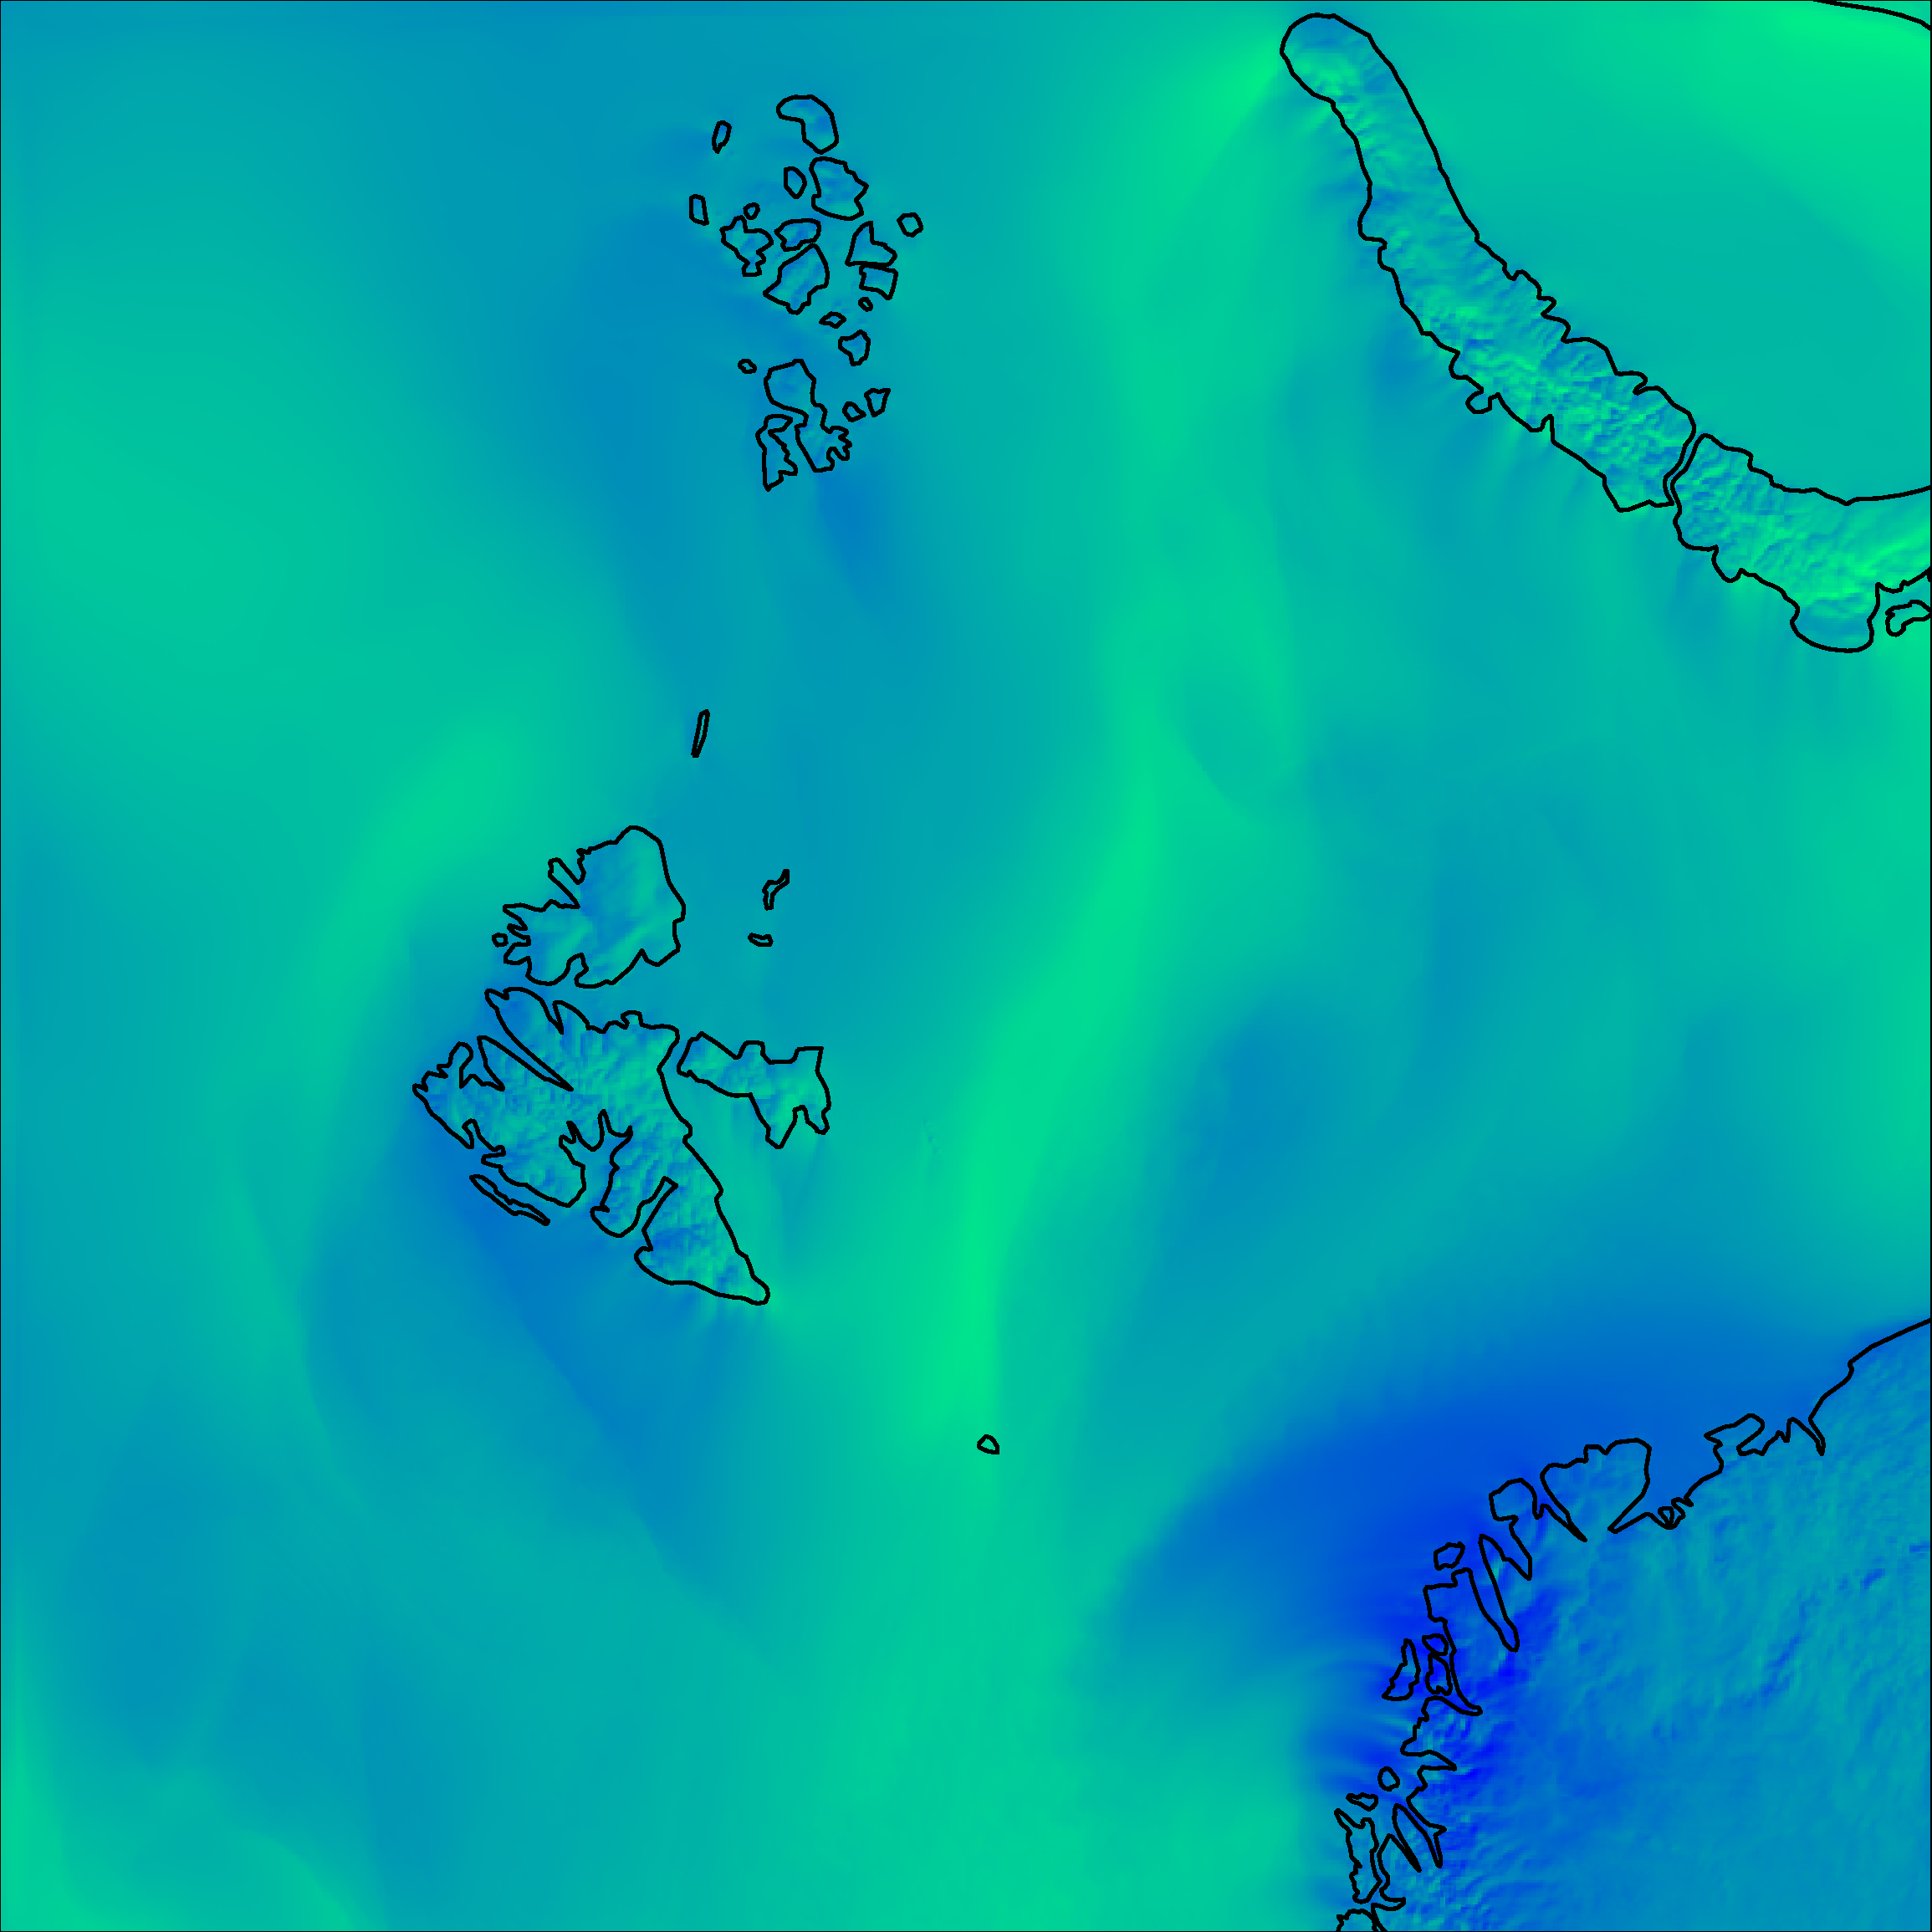
\includegraphics[width=.15\textwidth]{xwind.pdf}};
  \node[yshift = -0.4cm, xshift = 0.4cm] at (sample_stack) (stack5) {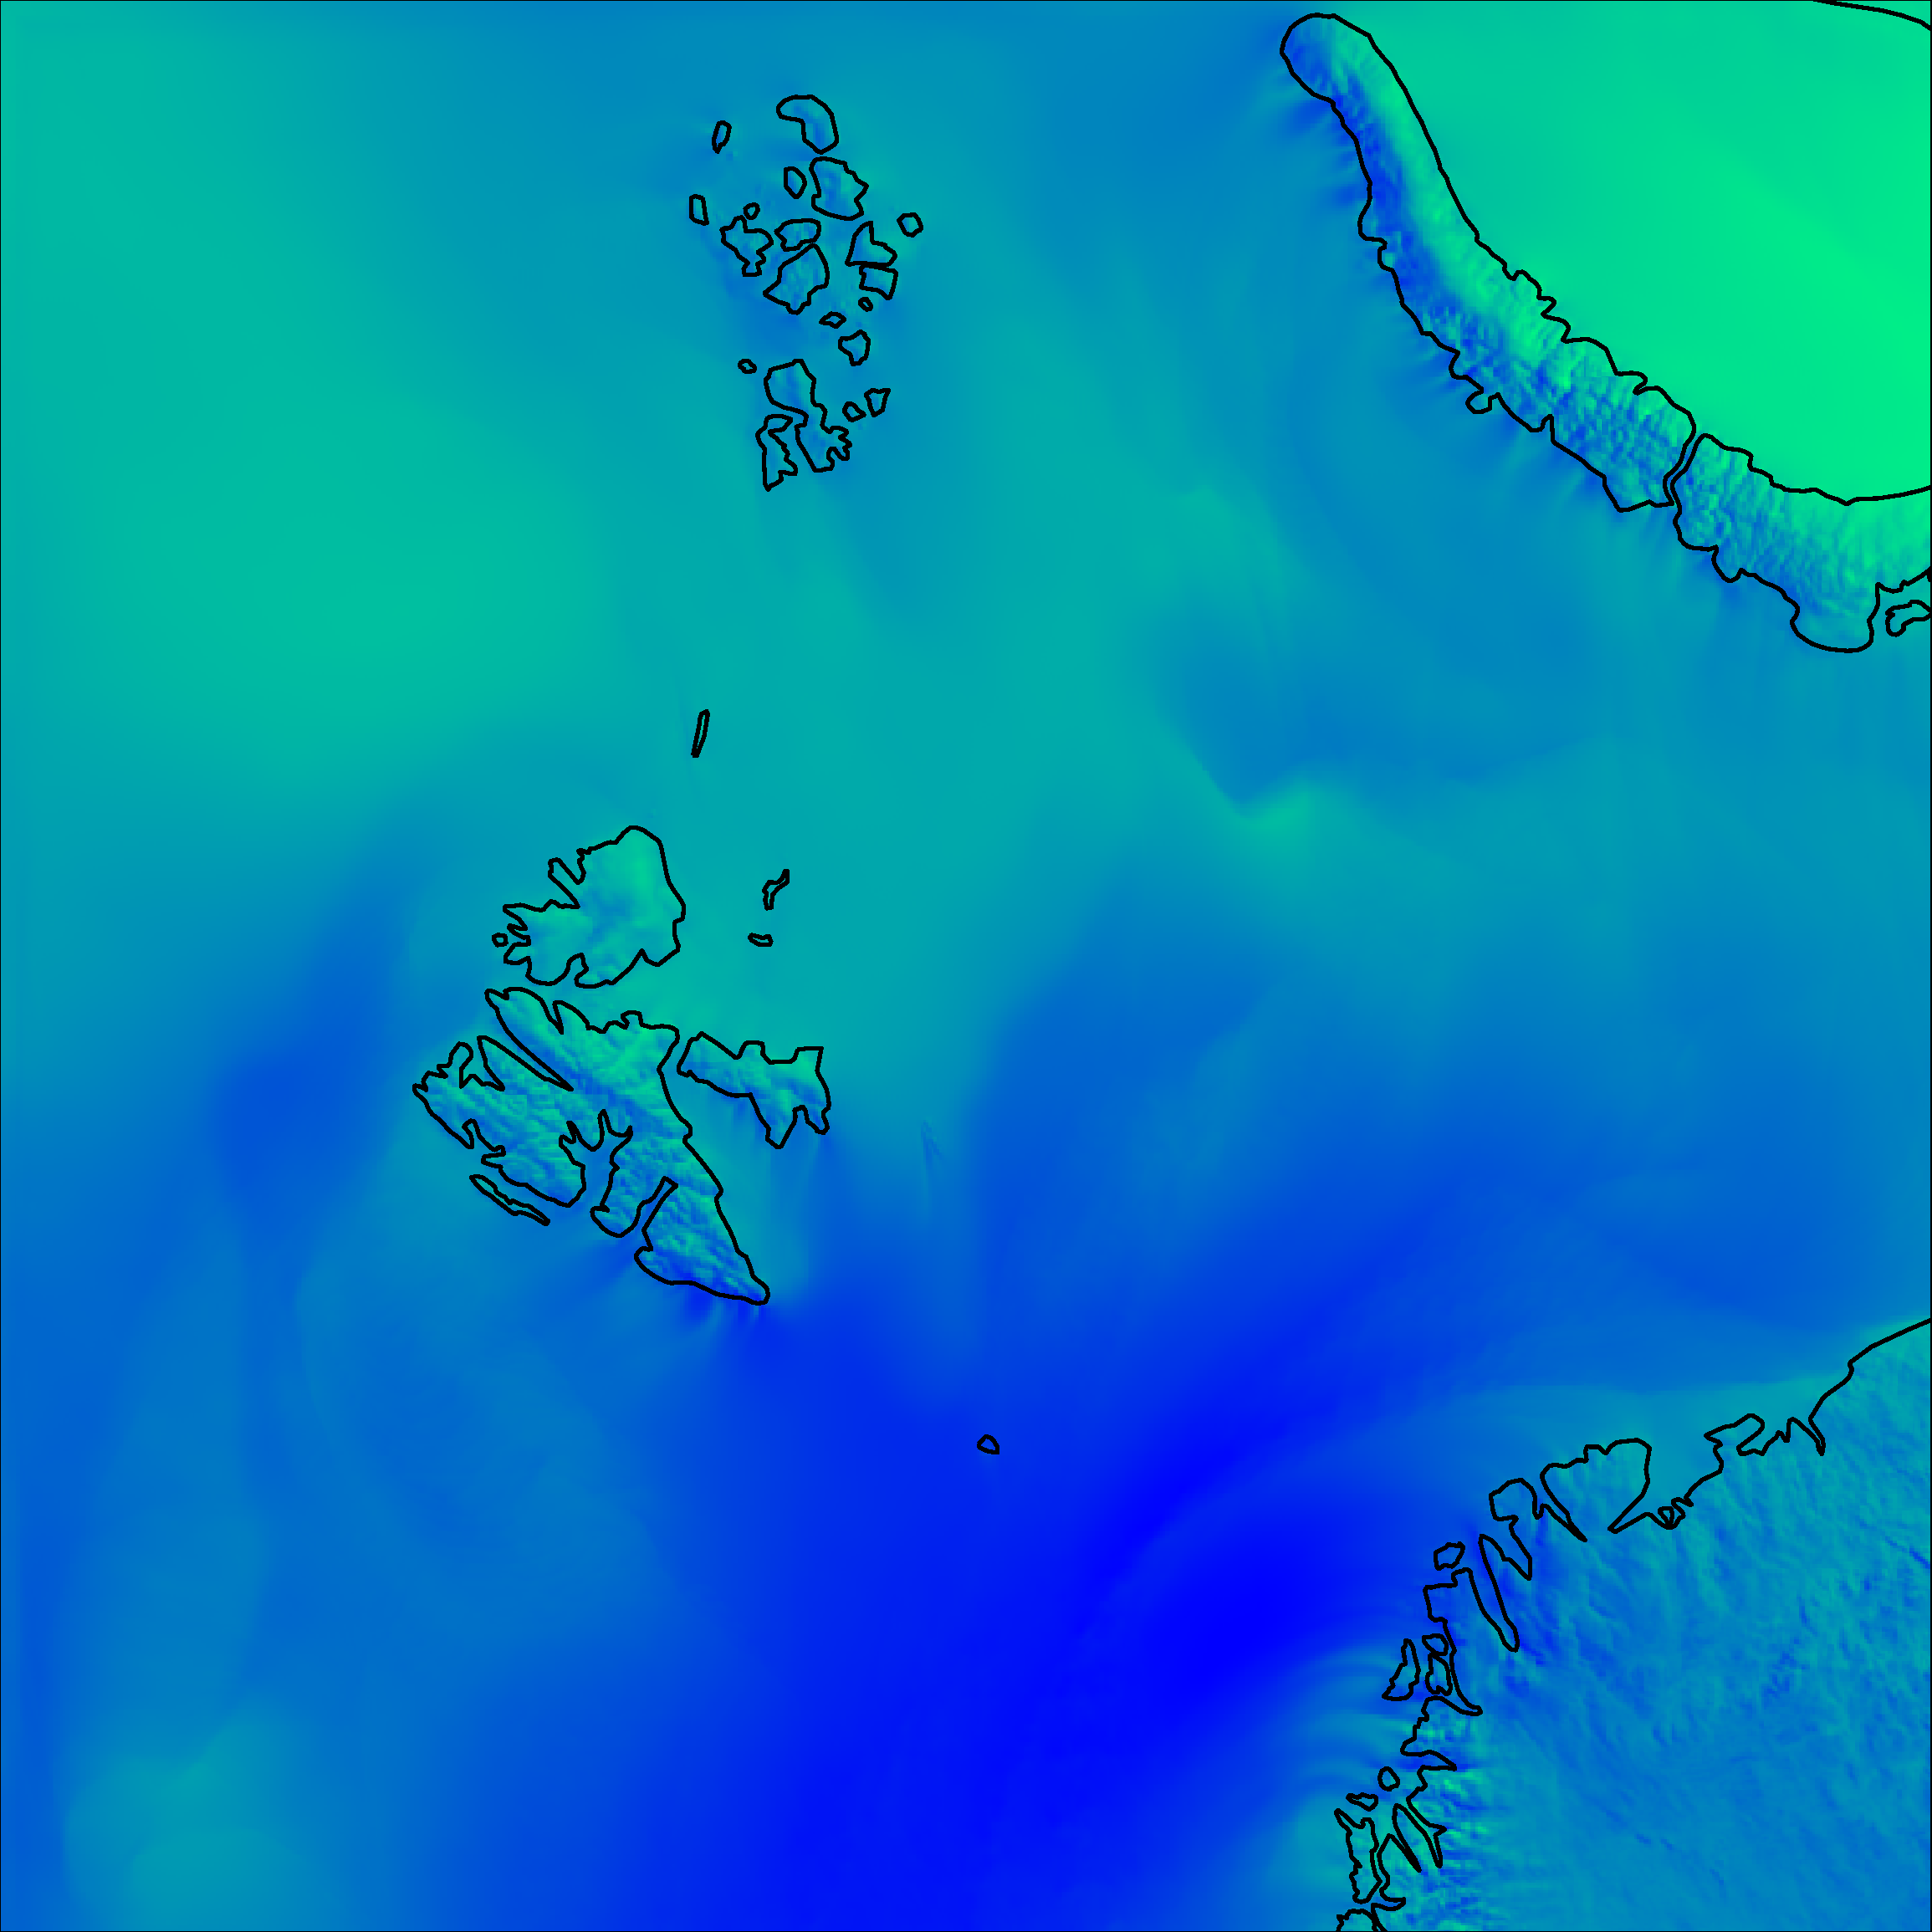
\includegraphics[width=.15\textwidth]{ywind.pdf}};
  \node[yshift = -0.5cm, xshift = 0.5cm] at (sample_stack) (stack6) {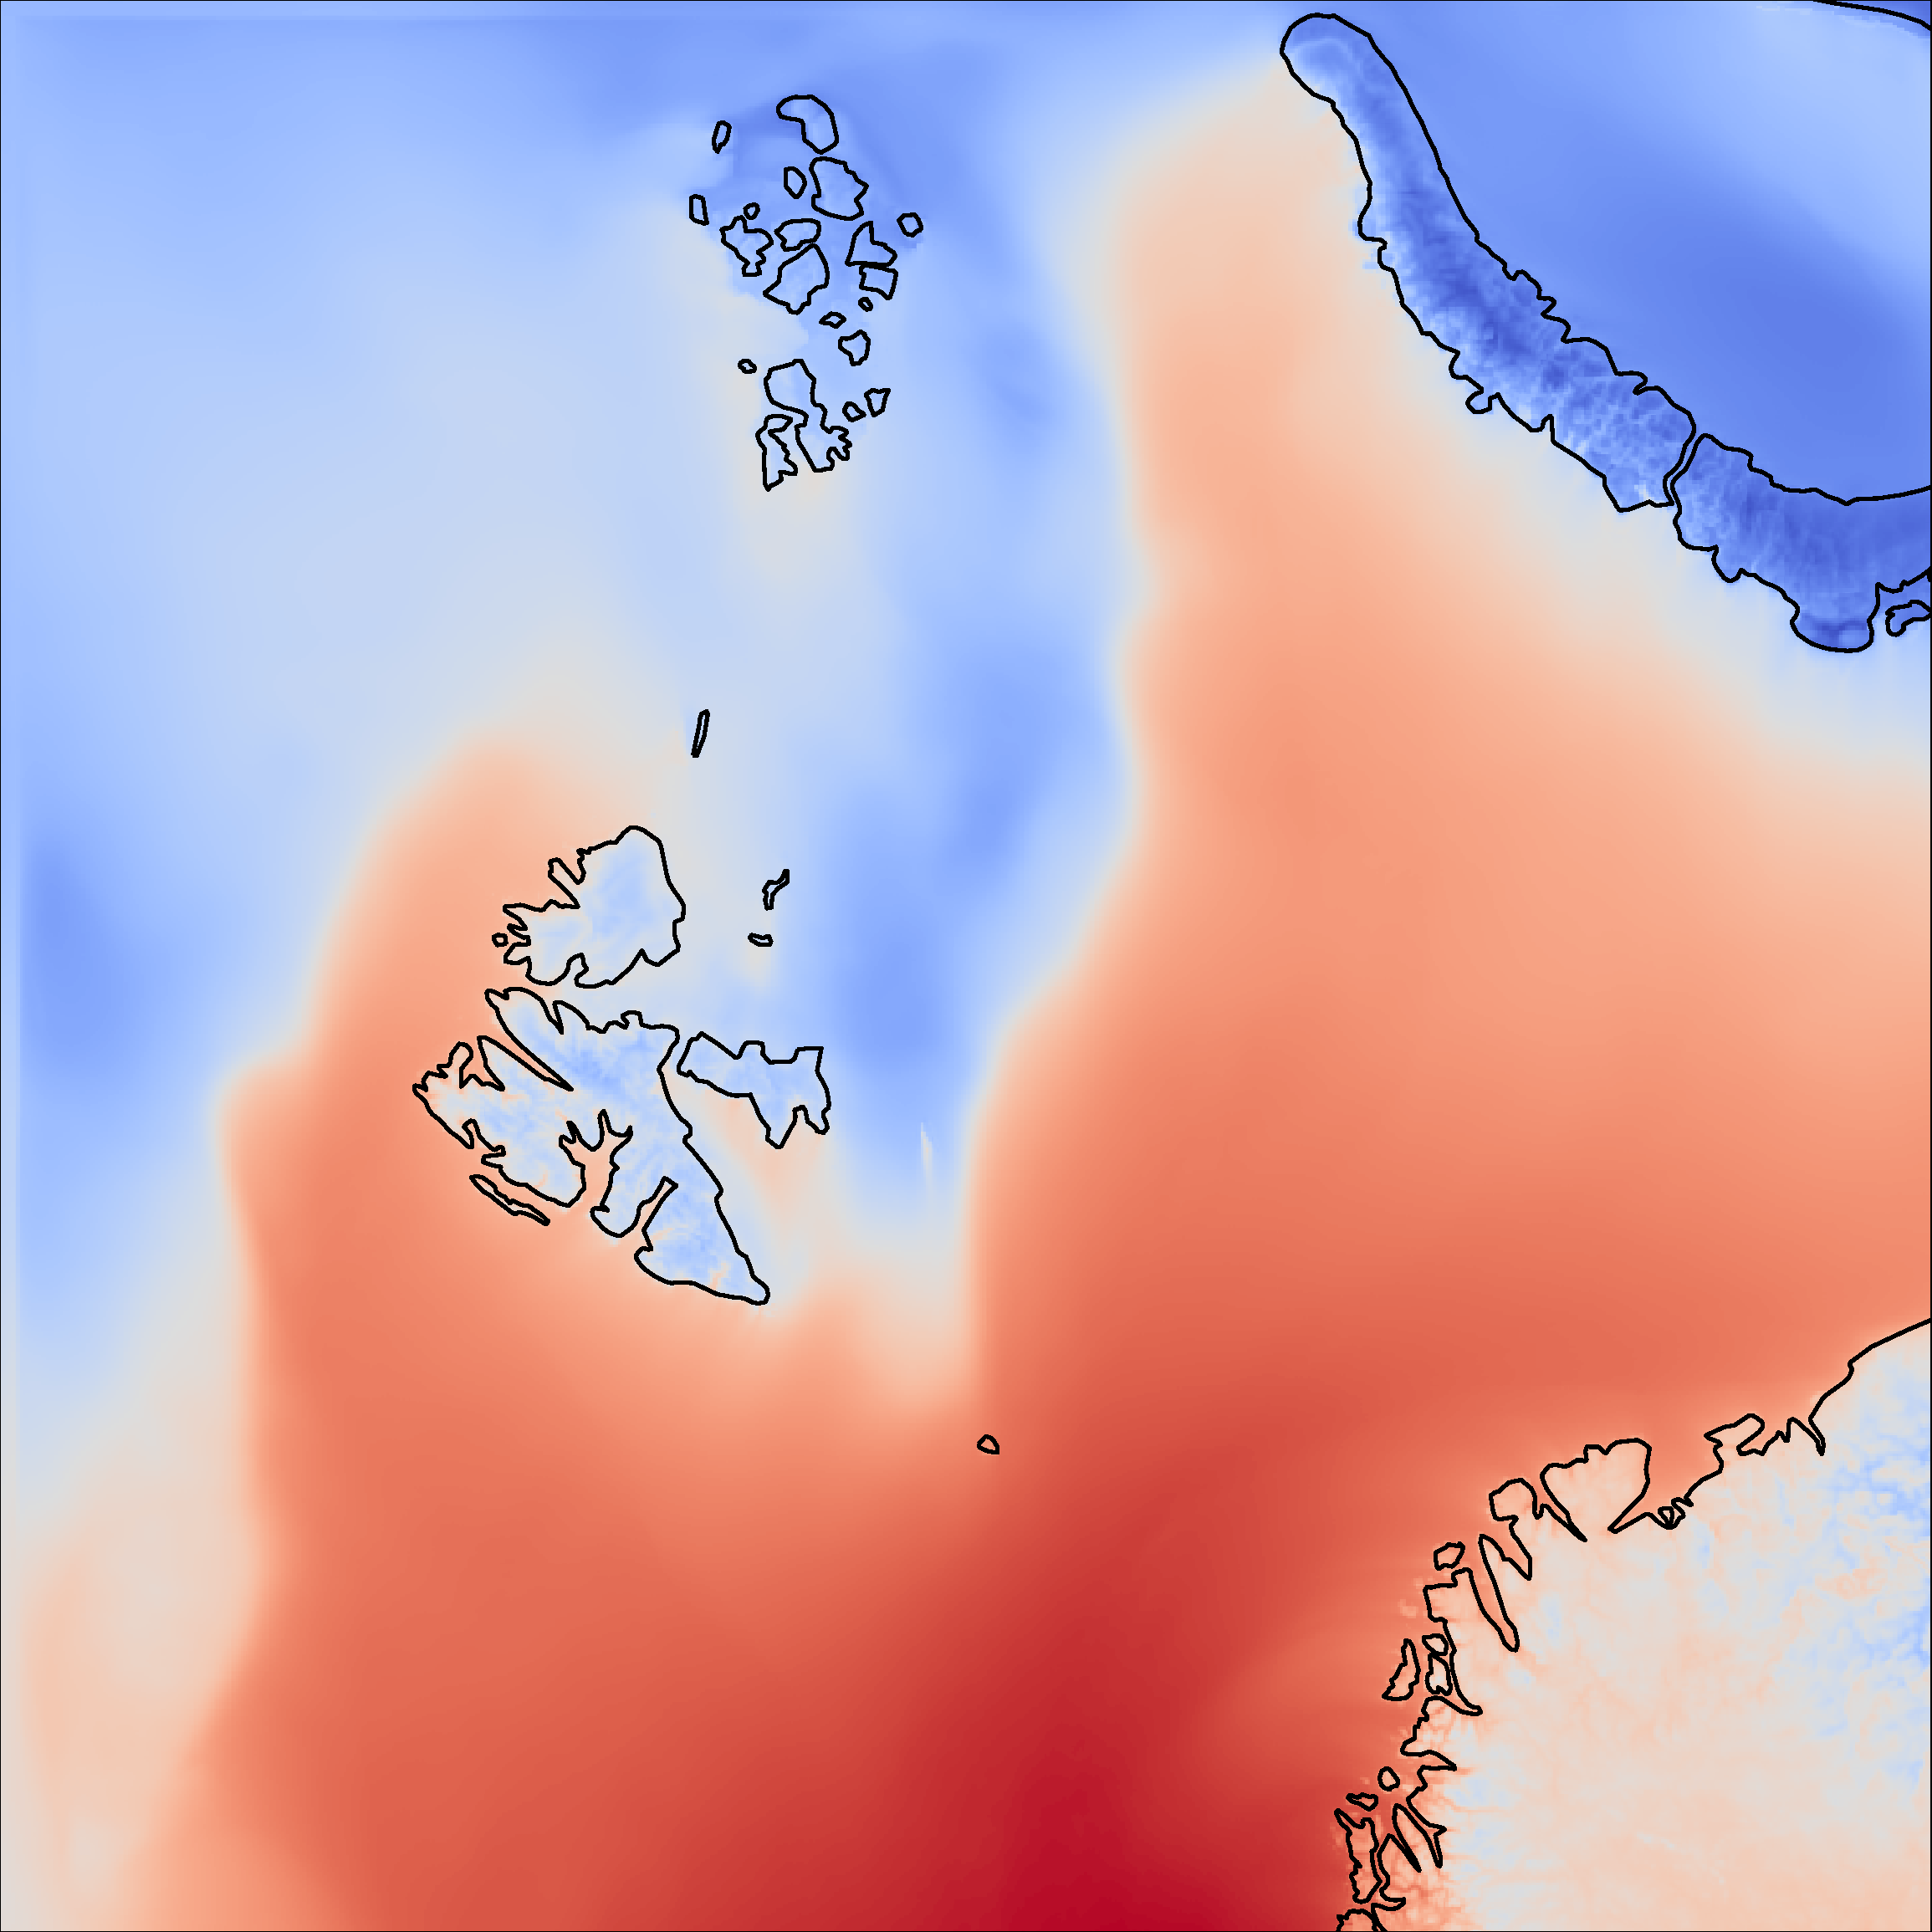
\includegraphics[width=.15\textwidth]{t2m.pdf}};
  
  \node[left = 1cm of sample_stack] (stack_name) {\large Sample};

  \node[below = 4cm of sample_stack, rectangle, draw=orange!50, fill=orange!20, thick, minimum width = 2cm, minimum height = 2cm, align = center] (unet) {U-NET};
 
  
  \draw [line width=0.8mm, -{Stealth[length=8mm, round]}, shorten >= 0.1cm, shorten <= 1.5cm] (sample_stack.south) -- (unet) node[midway, fill = white, anchor = center, text = black, yshift = -0.3cm] {\large Predictor variables};

  \node (sic_target) at (unet -| sic) {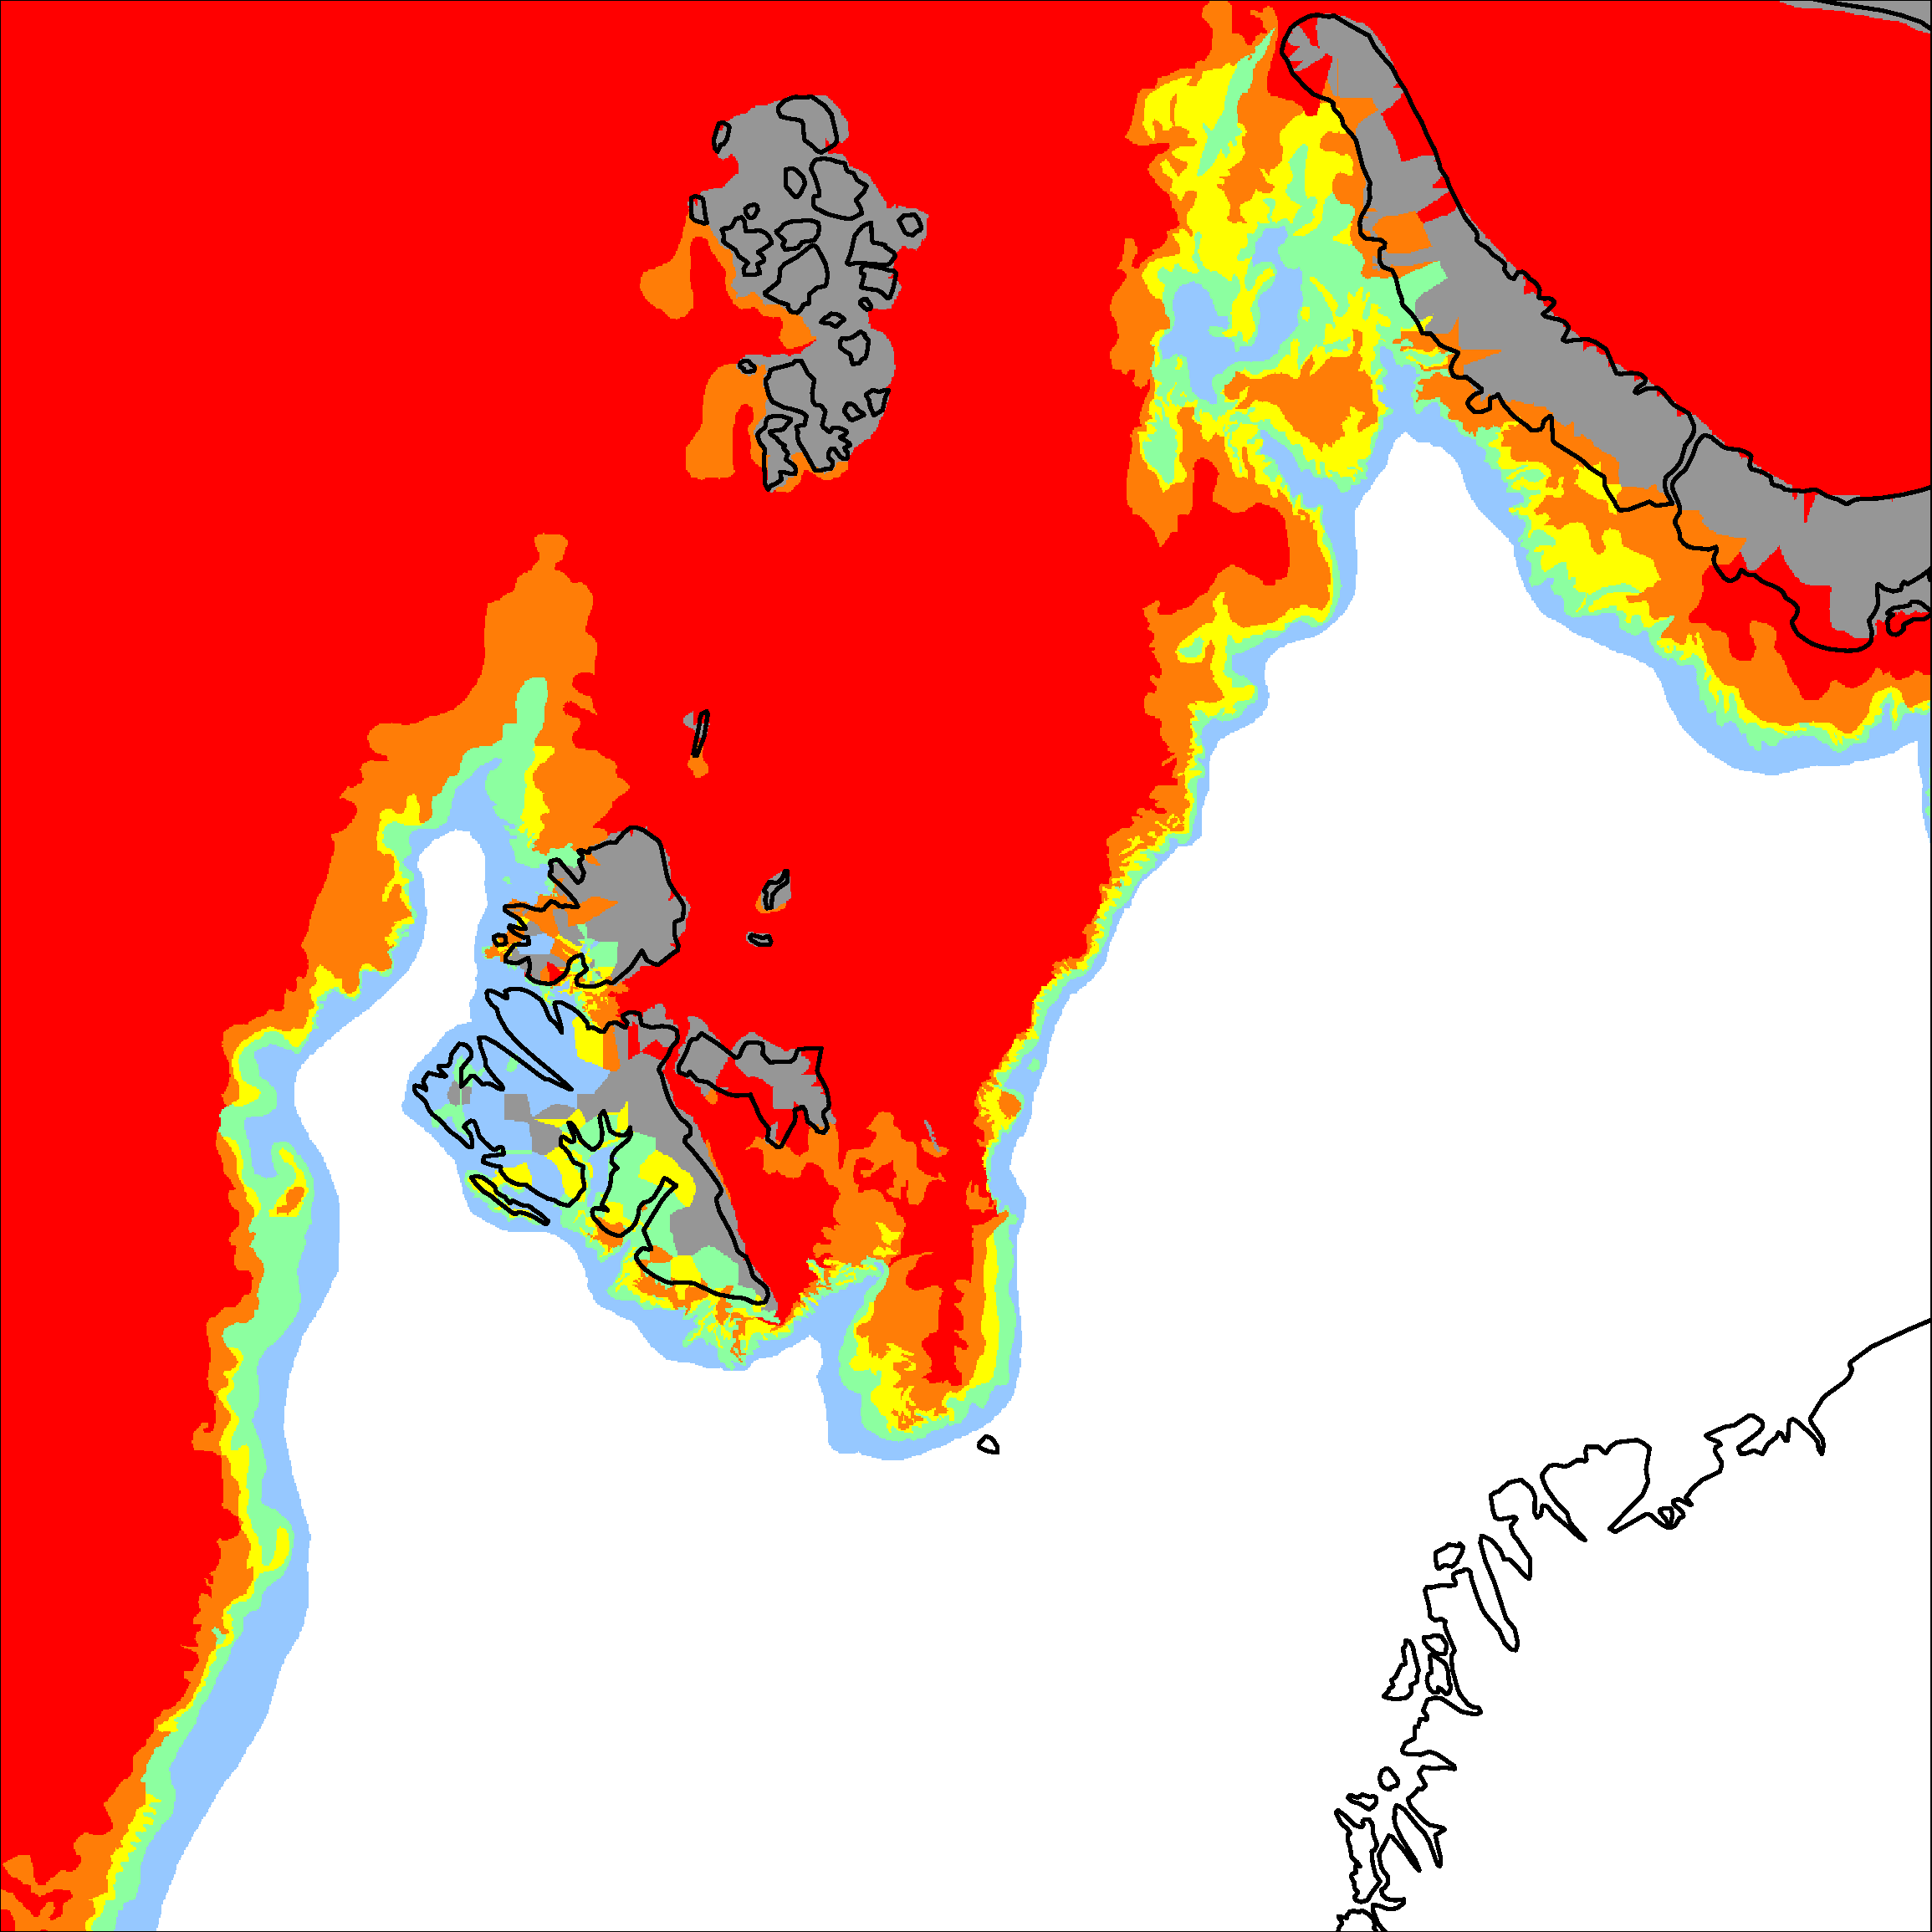
\includegraphics[width=.25\textwidth]{sic_target.pdf}};
  \node [above = 0cm of sic_target] (sic_target_name) {\large Target Ice Chart};
  \draw [line width=0.8mm, -{Stealth[length=8mm, round]}, shorten >= 0.1cm, shorten <= 0.1cm] (sic_target.east) -- node [midway, above = 0.2cm, xshift = -0.2cm] {\large Target variable} (unet.west);

  \node [inner ysep=3mm, below = 2cm of unet] (sic_pred) {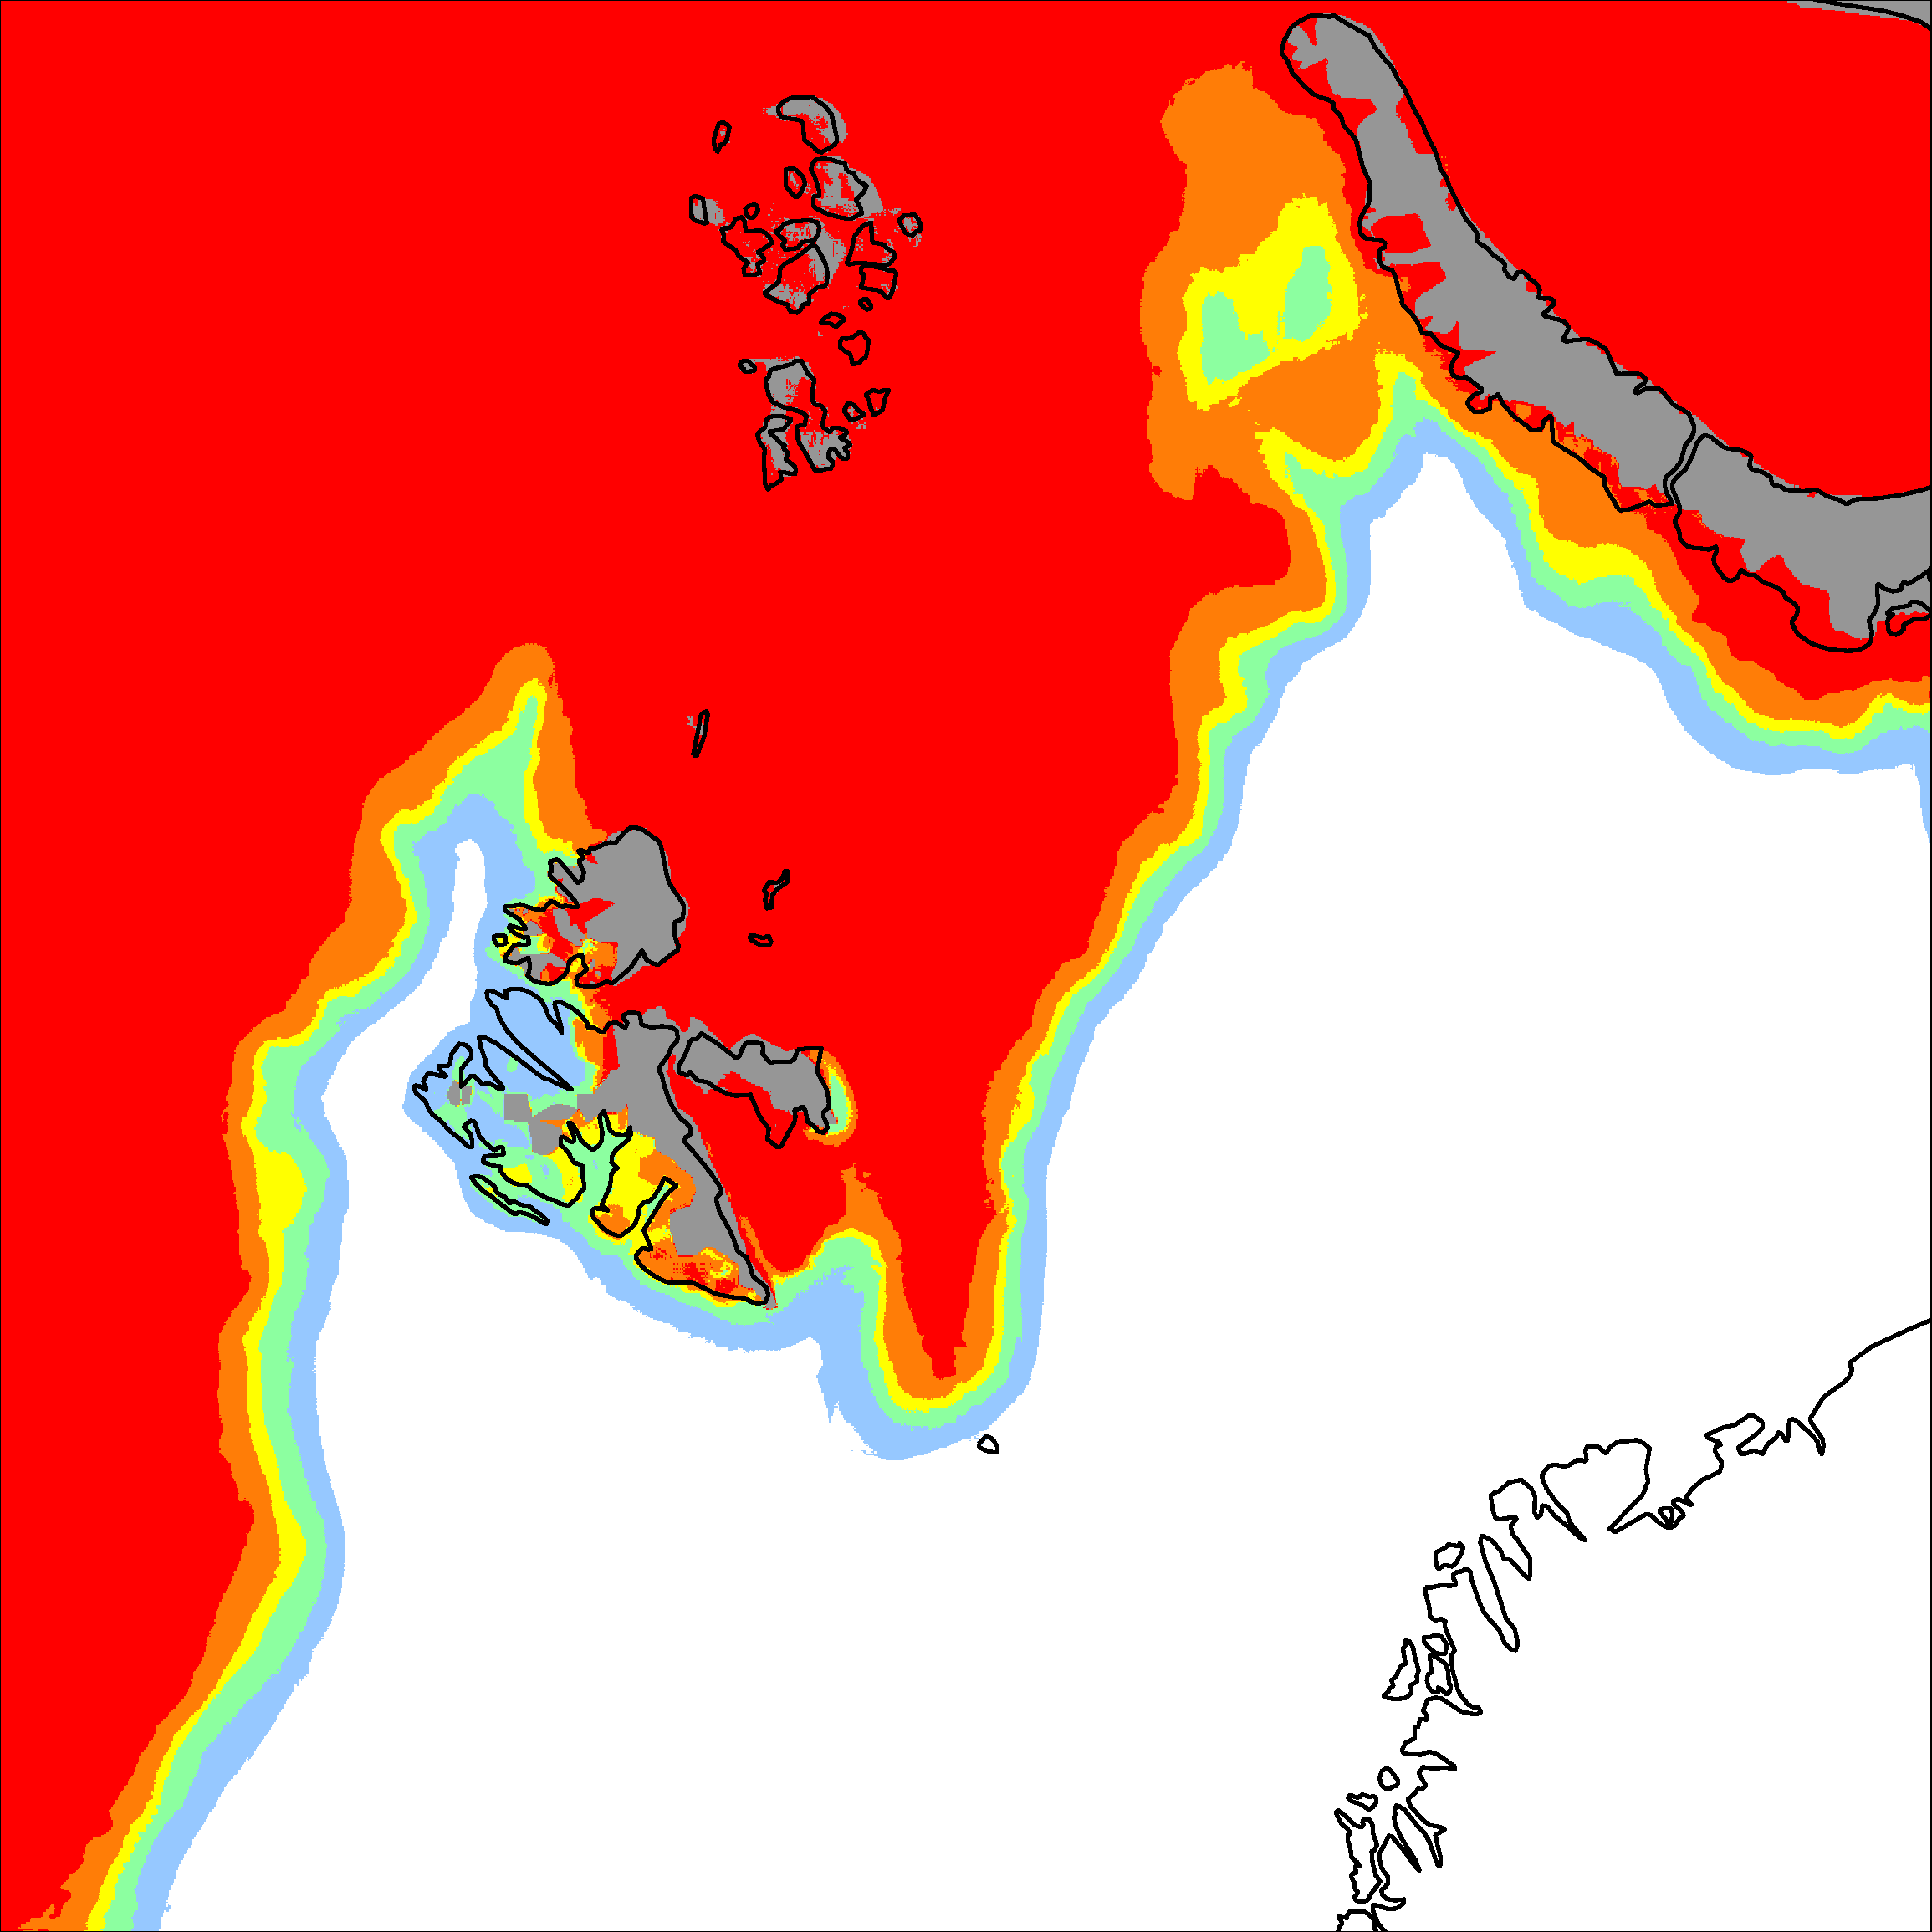
\includegraphics[width=.25\textwidth]{20220105.pdf}};
  \node [above = 0cm of sic_pred] (sic_pred_name) {\large Predicted Ice Chart};
  \draw [line width=0.8mm, -{Stealth[length=8mm, round]}, shorten >= 0.1cm, shorten <= 0.1cm] (unet.south) -- (sic_pred_name.north);

    
\end{tikzpicture}

\end{document}